%!TEX root=../documentation-bachlorthesis-speicherarchitektur-lstucker.tex
\cleardoublepage
\chapter{Evaluation}

\section{Soll-Kriterien festlegen}
Die gewählten Kriterien für die Evaluation wurden Zusammen mit dem Auftraggeber im Meeting festgelegt. In einen weiteren schritt, sind die einzelnen Kriterien nach ihren Logischen Zugehörigkeit hierarchisch geordnet und verfeinert (\refabb{abb:AHPKriterienbaum}). Die Überarbeitete Kriterien Auswahl wurde bei einen weiteren Meeting mit dem Auftraggeber besprochen und fixiert. 

Die Kriterien sind für die spätere Verweise die Verweise Hierarchisch-Nummeriert.

\begin{center}
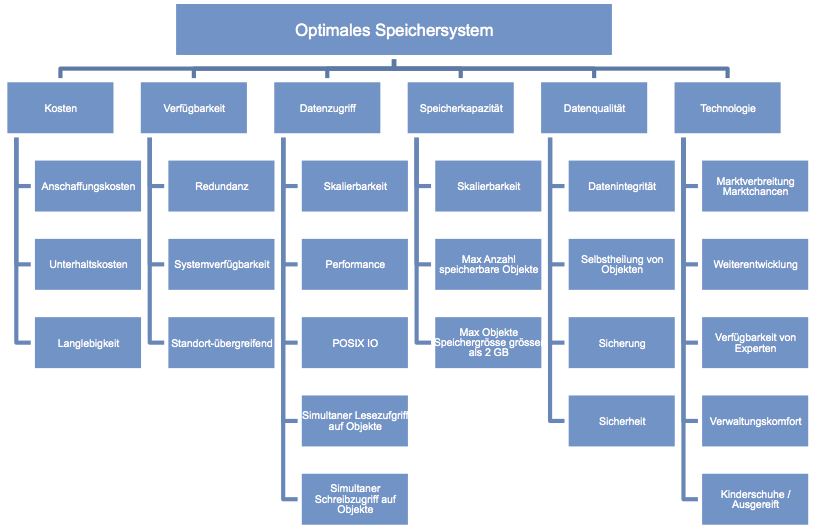
\includegraphics[width=\linewidth, keepaspectratio = true]{media/ahp_kirterienbaum.png}
\mycaption{figure}{\label{abb:AHPKriterienbaum} Optimales Speichersystem Kriterien}
\end{center}

\subsection{Haupt Soll-Kriterien festlegen}
Die Haupt-Kriterien sind auf der obersten Hierarchie Ebene und werden durch Ihre unter Kriterien definiert.
\setcounter{paragraph}{0}
\renewcommand\theparagraph{Soll-\arabic{paragraph}}
\paragraph{Kosten}\label{Soll-1}
Die Kosten sollen das Kostendach von ??? nicht überschreiten. 

\paragraph{Verfügbarkeit}\label{Soll-2}
Die Verfügbarkeit der Daten soll in Bezug auf die Szenerien die Verfügbarkeit erfüllen können. 

\paragraph{Datenzugriffe}\label{Soll-3}
Der Datenzugriff soll Skalieren können, dass heisst es soll möglich sein von mehren Webserver auf den Datenspeicher zugreifen zu können. Der Datenzugriff soll über POSIX IO oder über eine Dokumentiertes API erfolgen können.

\paragraph{Speicherkapazität}\label{Soll-4}
Die Speicherkapazität soll die Speicheranforderungen der Szenerien erfüllen können. Zudem sollen die Speicherung von Grossen Dateien bis mindestens 2 Gigabyte möglich sein.

\paragraph{Datenschutz}\label{Soll-5}
Der Datenschutz der Daten soll gewährleistet werden, dabei gilt das Haupt Augenmerk auf die Unveränderbarkeit der Gespeicherten Daten. Wichtig für den Auftraggeber ist ebenfalls das die Datengesichert werden können.

\paragraph{Technologie}\label{Soll-6}
asdf

\subsection{Unter Soll-Kriterien festlegen}
Die unter Kriterien mit den gleichen Nummer-Ebene gehören zusammen zur gleichen oben-Kriterien und werden später bei der Gewichtung der Kriterien nur untereinander direkt Verglichen.

\setcounter{paragraph}{0}
\renewcommand\theparagraph{Soll-1-\arabic{paragraph}}

\paragraph{Anschaffungskosten}\label{Soll-1-1}

\paragraph{Unterhaltskosten}\label{Soll-1-2}

\paragraph{Nachhaltigkeit}\label{Soll-1-3}

\setcounter{paragraph}{0}
\renewcommand\theparagraph{Soll-2-\arabic{paragraph}}

\paragraph{Redundanz}\label{Soll-2-1}
Die redundante Haltung der aktiven Daten, dass heisst der Daten die Aktive zugegriffen und manipuliert werden können, Dient zur Erhöhung der Verfügbarkeit der Daten bei einen Komponenten Ausfall. Die doppelt Haltung der Daten zur Sicherungszwecken, wie Archivierung wird nicht als redundant erachtet, da diese nicht direkt zu einer Erhöhung der System Verfügbarkeit ohne Menschliche Unterstützung führt. Die Speicherlösung sollte mindestens die Daten doppelt, wenn möglich dreifach Redundanz halten. 


\paragraph{Systemverfügbarkeit}\label{Soll-2-2}
Die Systemverfügbarkeit, wird durch Software oder Hardware Redundanz erreicht. Das System soll möglichst Redundant ausgelegt sein um eine Verfügbarkeit nach AEC-3 Standard zu erreichen.

\paragraph{Standort-übergreifend}\label{Soll-2-3}
Die aktive Daten sollen nach Möglichkeit an mindesten zwei Standorte verfügbar sein, um den Dienst bei einen Ausfall eines Rechenzentrums aufrecht zu erhalten können.

\setcounter{paragraph}{0}
\renewcommand\theparagraph{Soll-3-\arabic{paragraph}}

\paragraph{Skalierbarkeit}\label{Soll-3-1}
Die Speicherlösung sollte bei bedarf Ihren Speicher an bis zu 30 Serversysteme zur Verfügung stellen können.

\paragraph{Performance}\label{Soll-3-2}
Die Speicherlösung soll eine IO Performance von mindesten 27.31 MBit pro Sekunde haben.

\paragraph{POSIX IO}\label{Soll-3-3}
Die POSIX IO (inoffizielle Bezeichnung) ist eine Teil des POSIX Standards welche die IO Schnittstelle für POSIX Kompatible Applikationen definiert. Der Standard definiert unteranderem die Funktionen read(), write(), open(), close() inklisive deren Fehler Behandlung. Die Speicherlösung soll, für eine einfache Implementierung, nach Möglichkeit diesen Standard unterstützen. 

\paragraph{Simultaner Lesezugriff auf Objekte}\label{Soll-3-4}
Das gleichzeitige Lesen auf das selbe Objekte von zwei oder mehrere Serversysteme soll möglich sein.

\paragraph{Simulataner Schreibzugriff auf Objekte}\label{Soll-3-5}
Das gleichzeitige schreiben auf das selbe Objekte von zwei oder mehrere Serversysteme soll optional möglich sein.

\setcounter{paragraph}{0}
\renewcommand\theparagraph{Soll-4-\arabic{paragraph}}

\paragraph{Skalierbarkeit}\label{Soll-4-1}

\paragraph{Max Anzahl speicherbare Objekte}\label{Soll-4-2}
Das Speicherlösung soll die Anzahl Speicherbaren Objekten der Soll-Zenarien unterstützen. 

\paragraph{Max Objekte Speichergrösse grösser als 2 GB}\label{Soll-4-3}
Das Speichersystem muss die Speicherung von Objekten mit einer Speichergrösse von mindestenz 2 GigaByte unterstützen.

\setcounter{paragraph}{0}
\renewcommand\theparagraph{Soll-5-\arabic{paragraph}}

\paragraph{Datenintegrität}\label{Soll-5-1}
Die Datenintegrität der gespeicherten Daten soll gewährleistet sein.

\paragraph{Selbstheilung von Objekten}\label{Soll-5-2}
Die Selbstheilung von nicht mehr integer Daten soll nach Möglichkeit unterstützt werden. Diese Funktion ist bei der Verwaltung von grossen Datenmengen eine unterstützende Funktion.

\paragraph{Datensicherung}\label{Soll-5-3}
Die gespeicherten Daten soll mit einen Sicherungsverfahren gesichert werden können. Wenn die aktiven Daten nicht an zwei Standorten zur Verfügung gestellt werden können, wie in (\refsoll{Soll-2-3}) definiert, ist es zwingen erforderlich das die Sicherung an einen zweiten Standort erfolgen kann.

\paragraph{Datensicherheit}\label{Soll-5-4}
Die Datenberechtigung wird in der Applikation Implementiert, die Speicherlösung soll nach Möglichkeit Sicherstellen, das die Daten nicht von dritten Zugegriffen werden kann.

\setcounter{paragraph}{0}
\renewcommand\theparagraph{Soll-6-\arabic{paragraph}}

\paragraph{Marktverbreitung / Marktchancen}\label{Soll-6-1}
Die Speicherlösung soll im Markt verbreitet sein oder Tendenzen aufweisen die auf eine Verbreiterung im Markt in den nächsten fünf Jahren schliessen lässt.

\paragraph{Weiterentwicklung}\label{Soll-6-2}
Die Speicher Technologien welche aktive Weiterentwickelt werden soll hoher bewertet werden als Speicherlösung Technologie welche nicht mehr weiter gepflegt werden.

\paragraph{Verfügbarkeit von Experten}\label{Soll-6-3}
Die Verfügbarkeit von Experten Speicherlösungstechnologie soll gegeben sein. Dabei ist das Experten Wissen auch nach Verfügbarkeit nach Lokalität zu bewerten. Die Verfügbarkeit von Experten im Raum Schweiz ist höher zu werten als im Raum Europa.

\paragraph{Verwaltungskomfort}\label{Soll-6-4}
Die Speichertechnologie soll die geforderte Datenmenge mit möglichst geringen Aufwand komfortable verwalten lassen.

\paragraph{Kinderschuhe / Ausgereift}\label{Soll-6-5}
Die Speicher Technologie soll Ausgereift und Stabil laufen. Eine Implementierung von Beta Technologie ist nicht erwünscht.
Die Technologie soll Ausgereift sein, bzw. keine erst Implementierung.

\section{KO-Kriterien}
Die KO-Kriterien sind muss Kriterien die von einen Speichersystem erfüllt werden müssen. Speichersysteme welche die KO-Kriterien nicht erfüllen werden bei der AHP-Evaluation ausgeschlossen. Die KO-Kriterien wurde zusammen mit dem Auftraggeber besprochen und vereinbart.

\setcounter{paragraph}{0}
\renewcommand\theparagraph{KO-\arabic{paragraph}}

\paragraph{Dateigrösse bis 2 Gigibyte}\label{KO-1}
Die Speicherung von Dateien die eine Speichergrösse von 2 Gibibyte muss unterstützt werden.

\paragraph{Speicherkapazität Szenarien}\label{KO-2}
Die geforderten Speicherkapazitäten der Szenerien inklusive die benötigte Kapazität für die Redundanz muss von der Speicherlösung unterstützt werden.

\paragraph{Kosten Spannweite}\label{KO-3}
Die Kosten der teuersten Speicherlösung, darf nicht dreimal teuerer sein als die Günstigste Lösung.

\section{Auswahl der Alternativen / Vertreter}
Mit dem Auftraggeber wurde definiert, dass aus den Speicherlösung, SAN, NAS, Distributed Filesystem Cluster, Online Speicher und   Dedizierter Server Webserver einen Vertreter für die Evaluation ausgewählt werden soll. Die Lösungen wurden nach Marktverbreitung, Technologie Leader ausgewählt.

Die Alternativen/ Vertreter sind für die spätere Verweise die Verweise Nummeriert.

\setcounter{paragraph}{0}
\renewcommand\theparagraph{Al-\arabic{paragraph}}
\paragraph{Hetzner}\label{Al-1}
Dedizierte Webserver zählen im engeren Sinn nicht als reine Speicherlösungen, der Deutsche Hosting Anbieter Hetzner bietet jedoch Dedizierte Webserver mit einer Speicherkapazität welche die Anforderung an die Kapazität des Szenario 1 (siehe \refsec{Szenario-1}) erfüllen. Hetzner als Dedizierter Webserver Anbieter wurde ausgewählt, weil die bestehende Lösungen ebenfalls mit Hetzer Webserver realisiert ist. 

\paragraph{NetApp}\label{Al-2}
Als Vertreter für die NAS Speicherlösung wurde Netapp xxx ausgewählt. Die Firma Netapp gehört mit ihren NAS Speicherlösung zu den Markführer (siehe \refsec{MartkEtabliert}) und gelten als 

\paragraph{NetApp}\label{Al-3}


\paragraph{Open-Stack Cloud Storage}\label{Al-4}
Open-Stack 
Als Verteilte Speicherlösung wurde ursprünglich zu beginn der Arbeit Hadoop HDFS ausgewählt, jedoch haben eigene Recherchen ergeben, dass Hadoop HDFS eher für die Speicherung von grossen Daten welche mittels einen MapReduce Algorithmus verarbeitet werden. Als Alternative zu Hadoop HDFS, kristalisierte sich GlusterFS und OpenStack Cloud Storage. Die Entscheidung viel am Ende auf Open-Stack Cloud Storage, da diese bereits erfolgreich bei RackSpace einen grösseren Online Speicheranbieter betrieben wird und es eine vergleichbares API hat wie Amazon S3. Zudem wird OpenStack von namhaften Informatik Unternehmen unterstützt-


\paragraph{Amazon S3}\label{Al-5}
Amazon S3 wurde als Represetator für Online Speicherlösung gewählt. Amazon S3 ist gemäss \refsec{MartkEtabliert} einer der Etabliertesten wenn nicht die erfolgreichste Online Speicherlösung. Amazon betreibt mehre Rechenzentrum in der gesamten Welt, als Speicherlösung Standort wird Europa ausgewählt.


\subsection{Gewichtung der Soll-Kriterien mit AHP}

In diesen Abschnitt werden alle Soll-Kriteren der gleichen Hierarchie-Ebene bzw.  gleichen Unter-Kriterien paarweise mit einander Verglichen und mit der Skala \reftab{tab:Gewichtsberechnung} aus dem \refchap{kab:Entscheidungsfindung} Gewicht.

% Vergleich mit Kosten
\paragraph*{\refsoll{Soll-1} verglichen mit \refsoll{Soll-2} (\ref{Soll-1}/\ref{Soll-2})} 
Mit steigenden Anforderungen an die Verfügbarkeit steigen auch die Kosten. Der Betrieb einer Infrastruktur eines Service Anbieters muss Kostendecken sein. Einen Ausfall des System während definierten Zeiten in welches das System Online sein muss, hat ebenfalls Auswirkungen auf das Unternehmen. So kann es zum Image Verlust, zu Kunden Abgänge führen, oder die Zahlung von Entschädigung erfordern. Einen Datenverlust kann trotzt Sicherungskopie bei Grossen Datenmengen zeitintensive und kostspielig werden. Aus diesen Gründen ist eine gute Balance zwischen Kosten und Verfügbarkeit zu finden. Die Kosten sind deshalb im Vergleich zur Verfügbarkeit zwischen gleich und etwas grösser zu Gewichten.

\textbf{Gewichtung: 2}

\paragraph*{\refsoll{Soll-1} verglichen mit \refsoll{Soll-3} (\ref{Soll-1}/\ref{Soll-3})}
Die Unterkriterien von Datenzugriffe sind mit Skalierbarkeit der Datenzugriffe, Performance und usw. wichtige Entscheidungskriteren, dennoch sind diese im Gesamten im Vergleich zu den Kosten Kritikern etwas tiefer zu Gewichten. Grund dafür ist, dass der rentable Betrieb der Web-Applikation sichergestellt werden muss.

\textbf{Gewichtung: 3}

\paragraph*{\refsoll{Soll-1} verglichen mit \refsoll{Soll-4}}
Die Kosten und die Speicherkapazität sind gleich hoch zu Gewichten. Grund dafür ist, dass die Speicherlösung den rentablen Betrieb der Web-Applikation ermöglichen muss, zugleich muss jedoch sichergestellt werden, dass die geforderte Speicherkapazität vom Speichersystem erfüllt wird.

\textbf{Gewichtung: 1}

\paragraph*{\refsoll{Soll-1} verglichen mit \refsoll{Soll-5}}
Wie in den anderen Vergleiche ist sicherzustellen, das die Web-Applikation rentable Betrieben werden kann, aus diesen Grund sind möglichst tiefe Kosten erforderlich. Die Kosten sind deshalb in Vergleich zur Technologie erheblich Grösser zu Gewichten.

\textbf{Gewichtung: 5}

\paragraph*{\refsoll{Soll-1} verglichen mit \refsoll{Soll-6}}

\textbf{Gewichtung: 7}
% Vergleich mit Verfügbarkeit
\paragraph*{\refsoll{Soll-2} verglichen mit \refsoll{Soll-3}}
Aus Sicht des Anwenders ist die Verfügbarkeit der Daten höher zu Gewichten als möglichst schnellen Zugriff oder die Art und weise wie zugegriffen wird. Allerdings kann eine langes Zeitüberschreitung beim ausliefern der Daten für den Anwender ebenfalls als nicht Verfügbarkeit empfunden werden. Die Verfügbarkeit ist zwischen etwas Grösser bis erheblich Grösser zu Gewichten als der Datenzugriff.

\textbf{Gewichtung: 4}

\paragraph*{\refsoll{Soll-2} verglichen mit \refsoll{Soll-4}}
Zum Geschäftsmodell des Auftraggeber gehört unter anderem die Bereitstellung von Speicherkapazität für die Speicherung der Bilddaten seiner Kunden. Sind die Speicherkapazitäten ausgeschöpft ist es dem Auftraggeber nicht mehr möglich in diesen Geschäftsbereich weiter zu Wachsen. Aus diesen Grund ist die Verfügbarkeit etwas geringere zu Gewichten als die Speicherkapazität.

\textbf{Gewichtung: 1/3}


\paragraph*{\refsoll{Soll-2} verglichen mit \refsoll{Soll-5}}
sdsd
\paragraph*{\refsoll{Soll-2} verglichen mit \refsoll{Soll-6}}


% Vergleich mit Datenzugriffe
\paragraph*{\refsoll{Soll-3} verglichen mit \refsoll{Soll-4}}

\paragraph*{\refsoll{Soll-3} verglichen mit \refsoll{Soll-5}}

\paragraph*{\refsoll{Soll-3} verglichen mit \refsoll{Soll-6}}

% Vergleich mit Speicherkapazität
\paragraph*{\refsoll{Soll-4} verglichen mit \refsoll{Soll-5}}

\paragraph*{\refsoll{Soll-4} verglichen mit \refsoll{Soll-6}}

% Vergleich mit Datenschutz
\paragraph*{\refsoll{Soll-5} verglichen mit \refsoll{Soll-6}}




\begin{table}[htbp]
\caption{AHP Gewichtung Top Kriterien}
\begin{tabular}{|l|c|c|c|c|c|r|r|}
\hline
\multicolumn{ 1}{|c|}{} & \multicolumn{ 5}{c|}{Evalutations Matrix} & \multicolumn{1}{l|}{} & \multicolumn{1}{l|}{Gewicht} \\ \cline{ 2- 8}
\multicolumn{ 1}{|c|}{} & K & V & P & S & D & \multicolumn{1}{c|}{r} & \multicolumn{1}{c|}{w} \\ \hline
Kosten (K) & \textbf{1} & 2 & 3 & 1 & 1 & 1.131 & 0.226 \\ \hline
Verfügbarkeit (V) &  1/2 & \textbf{1} & 5 &  1/3 &  1/8 & 0.569 & 0.114 \\ \hline
Performance (P) &  1/3 &  1/5 & \textbf{1} &  1/4 &  1/7 & 0.257 & 0.051 \\ \hline
Speicherkapazität (S) & 1 & 3 & 4 & \textbf{1} &  1/2 & 1.071 & 0.214 \\ \hline
Datenqualität (D) & 1 & 8 & 7 & 2 & \textbf{1} & 1.972 & 0.394 \\ \hline  \hline
Ci & \multicolumn{1}{r|}{3.833} & \multicolumn{1}{r|}{14.200} & \multicolumn{1}{r|}{20.000} & \multicolumn{1}{r|}{4.583} & \multicolumn{1}{r|}{2.768} & 5 & 1 \\ \hline 
\end{tabular}
\label{AHPTop}
\end{table}

\subsubsection{Gewichtung Kosten}

Wie nach der Gewichtung und in der \reftab{tab:AHPKosten} zu entnehmen ist, haben die Unterhaltskosten, gefolgt von Langlebigkeit die höhere Gewichtung als die Anschaffungskosten.

Die Paarvergleiche im Detail:

\paragraph*{\refsoll{Soll-1-1} verglichen mit \refsoll{Soll-1-2} (\ref{Soll-1-1}/\ref{Soll-1-2})}
Die Betriebskosten sind der Hauptkostenfakor in der Lebenszeit eines Informations-Systems. Gemäss Gartner vielen die Weltweiten IT-Kosten im Jahr 2011 zu 20\% für die Computer Hardware und zu 43\% IT-Service an. Zudem Steigen die Kosten zum Beispiel von Disk Array Speicher nach Ablauf der ordentlichen von Hersteller gewährleisteten Wartung, wegen teuren weiterführenden Wartungsverträge stark an.
Aus diesen Grund sind die Anschaffung Kosten im vergleich zur Unterhaltskosten erheblich geringer zu Gewichten.

\textbf{Gewichtung: 1/5}

\paragraph*{\refsoll{Soll-1-1} verglichen mit \refsoll{Soll-1-3} (\ref{Soll-1-1}/\ref{Soll-1-3})}
Fällt die Langlebigkeit eines Systems, weil es technologisch veraltet ist oder weil die Kosten für Wartungsverträge nach Ablauf der ordentlichen Wartung im Vergleich zur neu Anschaffung unrentabel sind, kurz aus. Sind erneut Kosten in der Anschaffung und Migration der Daten notwendig. Aus diesen Grund sind die Anschaffungskosten im Vergleich zur Langlebigkeit etwas geringer zu Gewichten.

\textbf{Gewichtung: 1/3}


\paragraph*{\refsoll{Soll-1-2} verglichen mit \refsoll{Soll-1-3} (\ref{Soll-1-2}/\ref{Soll-1-3})}
Der Hauptkostenfakor in der Lebenzeit eines Information System sind die Betreibskosten, steigen diese Kosten Aufgrund hoher Wartungverträgekosten mit der Lebenspanne des Systems an, kann sich der Betrieb als unrentable herausstellen. Aus diesen Grund sind die Betriebskosten im Vergleich zu Langlebigkeit etwas grösser zu Gewichten.

\textbf{Gewichtung: 3}

\begin{table}[htbp]
\caption{AHP Kosten}
\begin{tabular}{|l|r|l|l|l|}
\hline
\multicolumn{ 5}{|c|}{\textbf{Kosten}} \\ \hline
 & \multicolumn{1}{l|}{\textbf{A}} & \textbf{U} & \textbf{L} & \textbf{Gewicht} \\ \hline
\textbf{Anschaffung (A)} & 1 & \multicolumn{1}{r|}{0,2} & \multicolumn{1}{r|}{0,333} & \multicolumn{1}{r|}{0,105} \\ \hline
\textbf{Unterhaltskosten (U)} & 5 & \multicolumn{1}{r|}{1} & \multicolumn{1}{r|}{3} & \multicolumn{1}{r|}{0,637} \\ \hline
\textbf{Langlebigkeit (L)} & 3 & \multicolumn{1}{r|}{0,333} & \multicolumn{1}{r|}{1} & \multicolumn{1}{r|}{0.258} \\ \hline
\textbf{Konsistenz Kennzahl} & 0.033  \\ \cline{1-2}
\end{tabular}
\label{tab:AHPKosten}
\end{table}

\subsubsection{Gewichtung Verfügbarkeit}

Wie nach der Gewichtung und in der \reftab{tab:AHPVerfügbarkeit} zu entnehmen ist, hat die Redundanz erheblich höher Gewichtung als die Systemverfügbarkeit und Standort-Übergreifende Verfügbarkeit.

Die Paarvergleiche im Detail:

\paragraph*{\refsoll{Soll-2-1} verglichen mit \refsoll{Soll-2-2} (\ref{Soll-2-1}/\ref{Soll-2-2})}
Die Daten eines Informationssystem sind dessen wertvollstes Gut, mit höherer Redundanz der Daten steigt auch die Verfügbarkeit der Daten.
Die Gesamt Verfügbarkeit hängt jedoch auch von der Verfügbarkeit der System Komponenten zusammen. Aus diesen Grund sollten die Daten System übergreifend Redundant sein um eine hohe Verfügbarkeit zu erreichen. Gemäss eigener Erfahrungen, ist die Zahl der Datenträger ausfälle höher als die restlichen Komponenten ausfälle eines Systems. Die Datenredundanz ist deshalb erheblich grösser zu Gewichten als die System Redundanz.

\textbf{Gewichtung: 5}

\paragraph*{\refsoll{Soll-2-1} verglichen mit \refsoll{Soll-2-3} (\ref{Soll-2-1}/\ref{Soll-2-3})}
Die Standortübergreifende Verfügbarkeit der Daten kann nur mit Redundanz der Daten erreicht werden, aus diesen Grund ist die Datenredundanz absolut höher zu Gewichten als die Standortübergreifende Verfügbarkeit.

\textbf{Gewichtung: 9}

\paragraph*{\refsoll{Soll-2-2} verglichen mit \refsoll{Soll-2-3} (\ref{Soll-2-2}/\ref{Soll-2-3})}
Die Standortübergreifende Verfügbarkeit des System kann, erreicht werden wenn die Daten auf mehre Standortverteilt werden und an diesen Standorten die Daten von einen System am selben Standort gelesen werden kann. Das zweite System könnte z.B. ein Typ gleiches sein, welches am zweiten Standort abgeschaltet ist und bei einen Ausfall des Hauptstandorts hochgefahren wird.
Um die Verfügbarkeit jedoch zu gewährleisten sollte keinen manuellen Eingriff erforderlich sein, da diese mit einen Unterbruch der Dienstleistung verbunden ist. Aus diesen Grund ist die Systemverfügbarkeit höher etwas bis erheblich höher zu Gewichten als die  Standortübergreifende Verfügbarkeit.

\textbf{Gewichtung: 4}

\begin{table}[htbp]
\caption{AHP Verfügbarkeit}
\begin{tabular}{|l|c|c|c|l|}
\hline
\multicolumn{ 5}{|c|}{\textbf{Verfügbarkeit}} \\ \hline
 & \multicolumn{1}{l|}{\textbf{R}} & \multicolumn{1}{l|}{\textbf{Sv}} & \textbf{St} & \textbf{Gewicht} \\ \hline
\textbf{Redundanz (R)} & 1 & 5 & \multicolumn{1}{r|}{9} & \multicolumn{1}{r|}{0,743} \\ \hline
\textbf{Systemverfügbarkeit (Sv)} & 1/5 & 1 & \multicolumn{1}{r|}{4} & \multicolumn{1}{r|}{0,194} \\ \hline
\textbf{Standort-Übergreifend (St)} & 1/9 & 1/4 & \multicolumn{1}{r|}{1} & \multicolumn{1}{r|}{0,063} \\ \hline
\textbf{Konsistenz Kennzahl} & 0,061 \\ \cline{1-2}
\end{tabular}
\label{tab:AHPVerfügbarkeit}
\end{table}

\subsubsection{Gewichtung Datenzugriff}

Wie nach der Gewichtung und in der \reftab{tab:AHPDatenzugriff} zu entnehmen ist, hat die Fähigkeit für Simultaner Lesezugriffe auf Objekte dicht gefolgt von Skalierbarkeit der Datenzugriffe die höchste Gewichtung. Gefolgt von Performance, der Unterstützung von POSIX IO. Die kleinste Gewichtung hat der Simultaner Schreibzugriff auf Objekte.


Die Paarvergleiche im Detail:

\paragraph*{\refsoll{Soll-3-1} verglichen mit \refsoll{Soll-3-2} (\ref{Soll-3-1}/\ref{Soll-3-2})}
Die Skalierung der Datenzugriff, dass heisst der Zugriff von mehren Systemen, ermöglicht es die Web-Applikation höher Redundant zu betreiben und die Verarbeitung der Bilddaten auf mehre Server zu Verteilen. Der maximale Datendurchsatz ist daher weniger bedeutend als dessen kostanz bei der Verteilung der Zugriffe auf mehere Server. Aus diesen Grund. Ein Speicherlösung welche schlechte Performance aufweist, skaliert jedoch in der Regel ebenfalls nicht. Aus diesen Grund ist die Skalierung der Datenzugriffe etwas grosser Gewichten als die Performance 

\textbf{Gewichtung: 3}

\paragraph*{\refsoll{Soll-3-1} verglichen mit \refsoll{Soll-3-3} (\ref{Soll-3-1}/\ref{Soll-3-2})}
Ist eine Zugriff auf die Daten über POSIX IO möglich, fällt allenfalls die Anpassung der Entwickelte Web-Applikation geringer aus als wenn er auf die Daten per API zugreifen muss. Für den Betrieb der Web-Applikation ist die Skalierung des Datenzugriffs sehr viel bis absolut bedeutender als die Methode des Datenzugriffs.

\textbf{Gewichtung: 8}


\paragraph*{\refsoll{Soll-3-1} verglichen mit \refsoll{Soll-3-4} (\ref{Soll-3-1}/\ref{Soll-3-4})}
Der Simultaner Lese Zugriff auf ein Objekt ermöglicht es, dass eine Bilddatei von mehren Server simultan gelesen werden kann und den Website Besuchern dargestellt werden kann. Wird diese nicht unterstützt ist es möglich das dem Webseiten Besucher die Bilddatei nicht dargestellt werden kann, wenn ein anderer Besucher die selbe Bilddatei betrachtet. Aus diesen Grund ist die Skalierung und der Simultane Lese Zugriff auf Objekten gleich bedeutend.

\textbf{Gewichtung: 1}


\paragraph*{\refsoll{Soll-3-1} verglichen mit \refsoll{Soll-3-5} (\ref{Soll-3-1}/\ref{Soll-3-5})}
Der Simultaner Schreibzugriff auf ein Objekt erlaubt es, dass eine Objekt simultan von zwei oder mehreren Systemen modifiziert werden kann. Die Web-Applikation des Auftraggeber führt jedoch keine Änderungen an einer Original Bilddatei durch sondern erstellt modifizierte Kopien. Aus diesen Grund ist Möglichkeit der gleichzeitigen Schreibzugriff auf ein Objekt absolut geringer zu Gewichten als die Skalierung des Datenzugriffs

\textbf{Gewichtung: 9}

\paragraph*{\refsoll{Soll-3-2} verglichen mit \refsoll{Soll-3-3} (\ref{Soll-3-2}/\ref{Soll-3-3})}
Für den Betrieb der Web-Applikation ist die Performance der Datenzugriffe erheblich bis sehr viel bedeutender als die Methode des Datenzugriffs.

\textbf{Gewichtung 6}

\paragraph*{\refsoll{Soll-3-2} verglichen mit \refsoll{Soll-3-4} (\ref{Soll-3-2}/\ref{Soll-3-4})}
Die Performance ist erheblich geringer bedeutend als der simultane Lesezugriff auf Objekte. Grund dafür ist das das gleiche Objekte von mehren Web-Server gelesen werden können um diese den Website Besuchern darstellen können 

\textbf{Gewichtung: 1/5}

\paragraph*{\refsoll{Soll-3-2} verglichen mit \refsoll{Soll-3-5} (\ref{Soll-3-2}/\ref{Soll-3-5})}
Aufgrund das keine Manipulationen an der Original Bilddatei durchgeführt wird, ist die Performance der Datenzugriff erheblich höher zu Gewichten als der Simultane Schreib zugriff auf Objekte 

\textbf{Gewichtung: 5}


\paragraph*{\refsoll{Soll-3-3} verglichen mit \refsoll{Soll-3-4} (\ref{Soll-3-3}/\ref{Soll-3-4})}
Die Zugriff Methode der Web-Applikation kann bei bedarf durch die Entwickler angepasst werden. Für den Betrieb der Web-Applikation ist daher die Zugriffs Methode auf die Bilddaten erheblich geringer bedeutend als der Simultane Lese Zugriff.

\textbf{Gewichtung: 1/5}


\paragraph*{\refsoll{Soll-3-3} verglichen mit \refsoll{Soll-3-5} (\ref{Soll-3-3}/\ref{Soll-3-5})}
 Aufgrund das keine Änderungen an Original Bilddateien durchgeführt werden, ist es für den Auftraggeber bedeutender, dass eine Zugriff über POSIX IO möglich ist.

\textbf{Gewichtung: 3}


\paragraph*{\refsoll{Soll-3-4} verglichen mit \refsoll{Soll-3-5} (\ref{Soll-3-4}/\ref{Soll-3-5})}
Die Webapplikation des Auftraggeber führt keine Änderungen an der Original Bilddatei durch, was den Simultaner Schreibzugriff auf Objekten für den Betrieb der Web-Applikation von geringer Bedeutung ist. Der Simultane Lesezugriff auf Objekten muss für den Betrieb der Web-Applikation möglich sein, damit die Bilddaten mehren Websitzungen dargestellt werden können. Aus diesen Grund ist es absolut grosser von Gewicht das ein Simultaner Lesezugriff möglich ist als der Simultaner Schreibzugriff.

\textbf{Gewichtung: 9}

\begin{table}[htbp]
\caption{AHP Gewichtung Datenzugriff}
\begin{tabular}{|l|c|c|c|c|c|l|}
\hline
\multicolumn{ 7}{|c|}{\textbf{Datenzugriff}} \\ \hline
 & \multicolumn{1}{l|}{\textbf{SK}} & \multicolumn{1}{l|}{\textbf{Pe}} & \multicolumn{1}{l|}{\textbf{POI}} & \multicolumn{1}{l|}{\textbf{L}} & \multicolumn{1}{l|}{\textbf{S  }} & \multicolumn{1}{l|}{\textbf{Gewicht}} \\ \hline
\textbf{Skalierbarkeit (Sk)} & 1 & 3 & 8 & 1 & 9 & 0,364 \\ \hline
\textbf{Performance (Pe)} & 1/3 & 1 & 6 & 1/5 & 5 & 0,158 \\ \hline
\textbf{POSIX IO (POI)} & 1/8 & 1/6 & 1 & 1/5 & 3 & 0,056 \\ \hline
\textbf{Simultaner Lesezugriff auf Objekte (L)} & 1 & 5 & 5 & 1 & 9 & 0,392 \\ \hline
\textbf{Simultaner Schreibzugriff auf Objekte (S)} & 1/9 & 1/5 & 1/3 & 1/9 & 1 & 0,031 \\ \hline
\textbf{Konsistenz Kennzahl} & 0,08  \\ \cline{1-2}
\end{tabular}
\label{tab:AHPDatenzugriff}
\end{table}

\subsubsection{Gewichtung Speicherkapazität}


Wie nach der Gewichtung und in der \reftab{tab:AHPSpeicherkapazität} zu entnehmen ist, hat die Skalierbarkeit zusammen mit Max Anzahl speicherbare Objekte die höchste Gewichtung. Die Möglichkeit zur Speicherung von Objekte grösser als 2 GiB hat die tiefste Gewichtung, da die mindestens Speichergrösse von 2 GiB bereits im KO Kriterium \ref{KO-1} festgelegt und es sich somit um ein Optionales Kriterien handelt wurde.

Die Paarvergleiche im Detail:

\paragraph*{\refsoll{Soll-4-1} verglichen mit \refsoll{Soll-4-2} (\ref{Soll-4-1}/\ref{Soll-4-2})}
Die Skalierung der Speicherkapazität ist gleich zu Gewichten wie die maximal Anzahl Speicherbare Objekt. Beides sind limitierende Faktoren, die bei erreichen der Grenze die Speicherung von neuen Objekten verunmöglichen. Erreicht man die Grenze der Speicherbaren Objekten,  kann der Vorhandene frei Speicherkapazität nicht für neue Objekte verwendet werden. Umgekehrt kann die Speicherkapazität nicht ausgebaut werden, können die frei Kapazität an Speicherbaren Objekten nicht dazu verwendet werden neue Objekte zu Speichern.

\textbf{Gewichtung: 1}

\paragraph*{\refsoll{Soll-4-1} verglichen mit \refsoll{Soll-4-3} (\ref{Soll-4-1}/\ref{Soll-4-3})}
Die Skalierbarkeit der Speicherkapazität, ist für den Betrieb sehr viel grösser zu Gewichten als die Maximale Speichergrösse für Objekte die grösser als 2 Gigibyte sind.

\textbf{Gewichtung: 7}

\paragraph*{\refsoll{Soll-4-2} verglichen mit \refsoll{Soll-4-3} (\ref{Soll-4-2}/\ref{Soll-4-3})}
Die maximale Anzahl speicherbare Objekte, ist für den Betrieb sehr viel grösser zu Gewichten als die Maximale Speichergrösse für Objekte die grösser als 2 Gigibyte sind.

\textbf{Gewichtung: 7}

\begin{table}[htbp]
\caption{AHP Gewichtung Speicherkapazität}
\begin{tabular}{|l|c|c|c|l|}
\hline
\multicolumn{ 5}{|c|}{\textbf{Speicherkapazität}} \\ \hline
 & \multicolumn{1}{l|}{\textbf{S}} & \textbf{A} & \textbf{O} & \textbf{Gewicht} \\ \hline
\textbf{Skalierbarkeit (S)} & 1 & \multicolumn{1}{r|}{1} & \multicolumn{1}{r|}{7} & \multicolumn{1}{r|}{0,467} \\ \hline
\textbf{Max Anzahl speicherbare Objekte (A)} & 1 & \multicolumn{1}{r|}{1} & \multicolumn{1}{r|}{7} & \multicolumn{1}{r|}{0,467} \\ \hline
\textbf{Max Objekt Speichergrosse grösser als 2 GiB (O)} & 1/7 & \multicolumn{1}{r|}{1/7} & \multicolumn{1}{r|}{1} & \multicolumn{1}{r|}{0.067} \\ \hline
\textbf{Konsistenz Kennzahl} & 0   \\ \cline{1-2}
\end{tabular}
\label{tab:AHPSpeicherkapazität}
\end{table}

\subsubsection{Gewichtung Datenschutz}

Wie nach der Gewichtung und in der \reftab{tab:AHPDatenschutz} zu entnehmen ist, hat das Kriterium Datensicherung gefolgt von Datenintegrität die höchste Gewichtung. Erheblich weniger Gewichtung haben Selbstheilung von Objekten und Datensicherheit.

Die Paarvergleiche im Detail:


\paragraph*{\refsoll{Soll-5-1} verglichen mit \refsoll{Soll-5-2} (\ref{Soll-5-1}/\ref{Soll-5-2})}
Damit das Speichersystem korrupte Objekte selbständig heilen kann, ist es erforderlich das die Objekte Redundant gespeichert sind und die Integrität der Gespeicherten Objekte geprüft werden kann. Die Integrität der Objekte wird dabei mit einen zuvor erstellten und gespeicherten Hash Prüfsumme verglichen. Aus diesen Grund ist die Datenintegrität erheblich höher zu Gewichten als die Selbstheilung von Objekten.

\textbf{Gewichtung: 5}

\paragraph*{\refsoll{Soll-5-1} verglichen mit \refsoll{Soll-5-3} (\ref{Soll-5-1}/\ref{Soll-5-3})}
Verliert man alle \gls{Primären-Daten} durch einen Hard-, Software Fehler oder durch einwirken von dritten, ist es unerlässlich das eine Sicherungskopie bereit steht um nicht den Total Datenverlust zu erleiden.
Eine weiter Gefahr von Datenverlust besteht, wenn die Datenintegrität nicht sichergestellt ist. Ist ein Objekt nicht mehr integer bzw. korrupt und wird diese vor der Sicherung nicht festgestellt, besteht die Gefahr eines Datenverlustes.
Der Verlust aller Daten ist jedoch schwerwiegender als der Verlust einzelner Daten.
Aus diesen Grund ist die Datenintegrität geringer zu Gewichten als die Datensicherung.

\textbf{Gewichtung: 1/3}

\paragraph*{\refsoll{Soll-5-1} verglichen mit \refsoll{Soll-5-4} (\ref{Soll-5-1}/\ref{Soll-5-4})}
Primär muss bei einer Webapplikation die Sicherheit der Daten innerhalb der Webapplikation sicher gestellt werden. Aus diesen Grund ist die Datenintegrität sehr viel grösser zu Gewichten als Sicherheit.

\textbf{Gewichtung: 7}

\paragraph*{\refsoll{Soll-5-2} verglichen mit \refsoll{Soll-5-3} (\ref{Soll-5-2}/\ref{Soll-5-3})}
Die Selbstheilung von Daten stellt sicher das alle Redundanten gespeicherten \gls{Primären-Daten} integer sind. Durch die Selbstheilung verringert sich das Risiko der eines Datenverlust zu erleiden. 
Der Verlust aller Daten ist jedoch schwerwiegender als der Verlust einzelner Daten.
Aus diesen Grund ist die Selbstheilung der Daten erheblich geringer zu Gewichten als die Datensicherung.

\textbf{Gewichtung: 1/5}

\paragraph*{\refsoll{Soll-5-2} verglichen mit \refsoll{Soll-5-4} (\ref{Soll-5-2}/\ref{Soll-5-4})}
Primär muss bei einer Webapplikation die Sicherheit der Daten innerhalb der Webapplikation sicher gestellt werden. Aus diesen Grund ist die Selbsheilung der Daten etwas grosser zu Gewichten als Sicherheit.

\textbf{Gewichtung: 3}

\paragraph*{\refsoll{Soll-5-3} verglichen mit \refsoll{Soll-5-4} (\ref{Soll-5-3}/\ref{Soll-5-4})}
Die Datensicherheit ist Primär auf der Web-Applikation Schicht zu gewährleisten und zu realisieren. Erfährt man einen Datenverlust durch einwirken von dritten, ist sicherzustellen das eine Sicherungskopie der Daten existiert. Aus diesen Grund ist die Sicherung der Daten sehr viel höher zu Gewichten als die Sicherheit.  

\textbf{Gewichtung: 7}

\begin{table}[htbp]
\caption{AHP Gewichtung Datenschutz}
\begin{tabular}{|l|c|c|c|c|l|}
\hline
\multicolumn{6}{|c|}{\textbf{Datenschutz}} \\ \hline
 & \multicolumn{1}{c|}{\textbf{I}} & \multicolumn{1}{c|}{\textbf{H}} & \multicolumn{1}{c|}{\textbf{B}} & \multicolumn{1}{c|}{\textbf{S}} & \multicolumn{1}{l|}{\textbf{Gewicht}} \\ \hline
\textbf{Datenintegrität (I)} & 1 & 5 & 1/3 & 7 & \multicolumn{1}{r|}{0,311} \\ \hline
\textbf{Selbstheilung von Objekten (H)} & 1/5 & 1 & 1/5 & 3 & \multicolumn{1}{r|}{0,097} \\ \hline
\textbf{Datensicherung (B)} & 3 & 5 & 1 & 7 & \multicolumn{1}{r|}{0,544} \\ \hline
\textbf{Datensicherheit (S)} & 1/7 & 1/3 & 1/7 & 1 & \multicolumn{1}{r|}{0,048} \\ \hline
\textbf{Konsistenz Kennzahl} & 0,084 \\ \cline{1-2}
\end{tabular}
\label{tab:AHPDatenschutz}
\end{table}

\subsubsection{Gewichtung Technologie}

Wie nach der Gewichtung und in der \reftab{tab:AHPTechnologie} zu entnehmen ist, hat das Kriterium Ausgereift mit abstand die höchste Gewichtung. Die zweit höchste Gewichtung weist die Weiterentwicklung auf gefolgt von Verfügbarkeit von Experten, Marktverbreitung/Marktchancen auf. Am wenigsten Gewicht hat der Verwaltungskomfort.

Die Paarvergleiche im Detail:


\paragraph*{\refsoll{Soll-6-1} verglichen mit \refsoll{Soll-6-2} (\ref{Soll-6-1}/\ref{Soll-6-2})}Eine Technologie die nicht mehr weiter Entwickelt wird, wird trotzt allfähiger aktuellen grosser Marktverbreitung, über kurz oder längere Zeit durch neuere Technologie aus dem Markt verdrängt. Beim entscheid einer neuen Lösung ist es deshalb wichtig, dass man sich für eine Technologie Entscheidet die nicht am Ende Ihrer Lebenszyklus steht. Aus diesen Grund ist die Marktverbreitung/Marktchance erheblich geringer zu Gewichten als die Weiterentwicklung.

\textbf{Gewichtung: 1/5}


\paragraph*{\refsoll{Soll-6-1} verglichen mit \refsoll{Soll-6-3} (\ref{Soll-6-1}/\ref{Soll-6-3})}
Durch eine hohe Marktverbreitung ist in der Regeln die Verfügbarkeit von Experten ebenfalls gegeben. Aus diesen Grund sind die Marktverbreitung und die Verfügbarkeit von Experten gleich zu Gewichten

\textbf{Gewichtung: 1}

\paragraph*{\refsoll{Soll-6-1} verglichen mit \refsoll{Soll-6-4} (\ref{Soll-6-1}/\ref{Soll-6-4})}
Ein Produkt welches hohen Verwaltungskomfort aufweist, jedoch wegen anderen Faktoren eine schlechte Marktverbreitung oder Marktchancen aufweist, ist für den längeren betrieb schlechter geeignet als eine Produkt mit weniger hohen Verwaltungskomfort. Die Marktverbreitung ist deshalb etwas hoher zu Gewichten als der Verwaltungskomfort.

\textbf{Gewichtung: 3}

\paragraph*{\refsoll{Soll-6-1} verglichen mit \refsoll{Soll-6-5} (\ref{Soll-6-1}/\ref{Soll-6-5})}
Für den Betrieb der Web-Applikation ist es wichtig das die Speicherlösung technisch und Betrieblich ausgereift sind. Die Marktverbreitung ist deshalb absolut geringer zu Gewichten als die Ausgereifheit der Speicherlösung.

\textbf{Gewichtung: 1/9}

\paragraph*{\refsoll{Soll-6-2} verglichen mit \refsoll{Soll-6-3} (\ref{Soll-6-2}/\ref{Soll-6-3})}
Eine Technologie, welche nicht mehr weiter entwickelt wird lauft Gefahr den Markt Anforderungen nicht mehr zu genügen und auf Dauer von neuen Technologien ersetzt zu werden. Der Rückgang der Marktanteile der Technologie hat auch zur Folge, dass der Nachwuchs sich in den alten Technologien weiter Bilden. Was wiederum zur Folge hat, dass die Anzahl Experten auf Dauer ebenfalls abnimmt. Aus diesen Grund ist die Weiterentwicklung erheblich höher zu Gewichten als die Verfügbarkeit von Experten.

\textbf{Gewichtung: 5}

\paragraph*{\refsoll{Soll-6-2} verglichen mit \refsoll{Soll-6-4} (\ref{Soll-6-2}/\ref{Soll-6-4})}

Die Weiterentwicklung ist für den Langezeit betrieb wichtiger als der Verwaltungskomfort. Bestehende Schwächen im Verwaltungskomfort, könnten in Weiterentwickelten Versionen behoben oder verbessert sein. Die Weiterentwicklung wird deshalb für den langzeit Betrieb sehr höher gewichtet als der Verwaltungskomfort.

\textbf{Gewichtung: 7}

\paragraph*{\refsoll{Soll-6-2} verglichen mit \refsoll{Soll-6-5} (\ref{Soll-6-2}/\ref{Soll-6-5})}
Für den Betrieb der Web-Applikation ist es wichtig, dass die Speicherlösung technisch und Betrieblich ausgereift sind. Die Weiterentwicklung ist deshalb erheblich geringer zu Gewichten als die Ausgereifheit der Speicherlösung.

\textbf{Gewichtung: 1/5}


\paragraph*{\refsoll{Soll-6-3} verglichen mit \refsoll{Soll-6-4} (\ref{Soll-6-3}/\ref{Soll-6-4})}
Biete eine Speicherlösung einen hohen Verwaltungskomfort, können die Verwaltung in der Regel schneller und von weniger gut geschulten Personal durchgeführt werden. Folglich ist verringert sich die Abhängigkeit zu Experten. Für die Konzeption, Inbetriebnahme, spätere Optimierung und Problemlösungen der Speicherinfrastruktur ist man in der Regeln weiterhin auf das Wissen von Experten angewiesen. Aus diesen Grund ist es wichtig das der Zugriff auf Experten Wissen gegeben ist. Die Verfügbarkeit von Experten ist deshalb, erheblich höher zu Gewichten als der Verwaltungskomfort. 

\textbf{Gewichtung: 5}

\paragraph*{\refsoll{Soll-6-3} verglichen mit \refsoll{Soll-6-5} (\ref{Soll-6-3}/\ref{Soll-6-5})}
Für den Betrieb der Web-Applikation ist es wichtig das die Speicherlösung technisch und Betrieblich ausgereift sind. Ist eine Produkt nicht ausgereift, bzw. verfügt über massive Mängeln die einen Betrieb gefährden, kann diese nicht gänzlich durch Experten Wissen kompensiert werden. Die Verfügbarkeit von Experten ist deshalb sehr viel geringer zu Gewichten als die Ausgereifheit der Speicherlösung.

\textbf{Gewichtung: 1/7}

\paragraph*{\refsoll{Soll-6-4} verglichen mit \refsoll{Soll-6-4} (\ref{Soll-6-3}/\ref{Soll-6-5})}
Für den Betrieb der Web-Applikation ist es wichtig das die Speicherlösung technisch und Betrieblich ausgereift sind. Der beste Verwaltungskomfort, bring am Ende nichts, wenn das Produkt durch Mängeln den Betrieb gefährdet.

Der Verwaltungskomfort ist deshalb absolut geringer zu Gewichten als die Ausgereiftheit der Speicherlösung.

\textbf{Gewichtung: 1/9}

\begin{table}[htbp]
\caption{AHP Gewichtung Technologie}
\begin{tabular}{|l|c|c|c|c|c|r|}
\hline
\multicolumn{ 7}{|c|}{\textbf{Technologie}} \\ \hline
 & \textbf{M} & \textbf{W} & \textbf{E} & \textbf{V} & \textbf{A} & \multicolumn{1}{l|}{\textbf{Gewicht}} \\ \hline
\textbf{Marktverbreitung/Marktchancen (M)} & 1 & 1/5 & 1 & 3 & 1/9 & 0.064 \\ \hline
\textbf{Weiterentwicklung (W)} & 5 & 1 & 5 & 7 & 1/5 & 0.238 \\ \hline
\textbf{Verfügbarkeit von Experten (E)} & 1 & 1/2 & 1 & 5 & 1/7 & 0.079 \\ \hline
\textbf{Verwaltungskomfort (V)} & 1/3 & 1/7 & 1/2 & 1 & 1/9 & 0.031 \\ \hline
\textbf{Ausgereift (A)} & 9 & 5 & 7 & 9 & 1 & 0.588 \\ \hline
\textbf{Konsistenz Kennzahl} & \multicolumn{1}{r|}{0.094}  \\ \cline{1-2}
\end{tabular}
\label{AHPTechnologie}
\end{table}


\section{Analyse Alternativen auf KO-Kriterien}

\section{Daten Sammeln}
\subsection{\ref{Al-1}: Hetzner Server}
Hetzner ist einer der grössten Hosting Anbieter in Deutschland und bietet seit 1997 für Unternehmen und Privat Personen Hosting-Produkte an. In den Vergangenen Jahren hat Hetzer diverse Computer-Magazin Auszeichnungen bekommen. Hetzner betreibt in Deutschland mehre Rechenzentren die mehrfach Redundant an das Internet Angeschlossen sind.

\paragraph{Speicherkapazität}
Der Grösste Dezidierter Server welche Hetzner in seinen Produkte Katalog führt, ist der Root Server XS 29. Der XS 29 ist mit 15 mal 3 Terabyte SATA Festplatten ausgerüstet. Mit dem zusätzlich eingebauten Hardware RAID Kontroller lassen, sich die 15 Festplatten zu einen RAID zusammen fügen.
Als CPU hat der Server einen Intel Xeon E3-1245 Quad-Core eingebaut und Verfügt über 16 Gigabyte Hauptspeicher. 

Die Max Grösse einer Datei ist von Dateisystem abhängig. ext3 oder "third extended filesystem" genannt, ist bei den meisten bekannten Linux Distributoren das Standard Dateisystem. Die maximale grösse einer Datei hängt von der verwendeten Blockgrösse ab. Nach eigener Test ist die Standard Blockgrösse bei Debian, Ubuntu, Red Hat und Suse 4 Kibibyte, gross. Bei einer Blockgrösse von 4 Kibibyte, kann eine Datei maximal 2 Tebibyte und das Dateisystem 16 Tebibyte gross sein. \cite{Card1993}

Die Maximale Anzahl an Objekte, hängt von der grösse des Dateisystems ab. Bei einen 16 Tebibyte ist mit der Standard Konfiguration maximal 17'592'186'044'416 Objekte. 

\paragraph*{Verfügbarkeit}
Die RAID-5 Konfiguration mit dem 15 Festplatten im RAID bietet mit 38,192 Tebibyte gemäss \refeqlb{eqn:MaxSpeicherkapazitätHeztner} bei einfacher Redundanz die grösste mögliche Speicherkapazität. Wegen der möglicherweise langen Wiederherstellungs-Zeit (MTTR) dieser Konfiguration, ist man darauf angewiesen, dass der Ausfall durch die eigene Überwachungssystem erkannt und nach Benachrichtigung des Hetzner Support die defekte Festplatte rasch ausgetauscht wird. Die Festplatten selber sind während des Betriebs austauschbar, es ist somit kein Unterbruch des Betriebs erforderlich.

Der eingesetzte LSI RAID Kontrolle lässt auch die Konfiguration einer Hot-Spare Festplatte zu. Eine Host-Spare Festplatte ist eine leere ungenutzte Festplatte, die bei einen Ausfall einer Festplatte im RAID automatisch die defekte Festplatte ersetzt. 

Da es sich nur um ein Server System handelt, ist eine Standort-übergreifende Verfügbarkeit der Daten nicht möglich.


\begin{equation}
\mbox{Anzahl Server} = (15 -1)* 2,728 \mathrm{\ TiB}=  38,192 \mathrm{\ TiB}
\label{eqn:MaxSpeicherkapazitätHeztner}
\end{equation}

\begin{equation}
\mbox{Anzahl Server} = (15 -1-1)* 2,728 \mathrm{\ TiB}=  35,464 \mathrm{\ TiB}
\label{eqn:MaxSpeicherkapazitätHeztnerHotspare}
\end{equation}

\paragraph*{Datenzugriff}
Der Datenzugriff findet lokal über POSIX IO statt, dass heisst das die Web-Applikation auf dem selben Server betrieben wird. 

Der Lese Zugriff und Schreibzugriff ist auf den Server begrenzt. Theoretisch könnte der Speicher mit Protokollen wie NFS zwischen, mehreren Systemen geteilt werden. Es handelt sich jedoch beim System um einen Miete Server, es kann deshalb nicht davon ausgegangen werden, das weitere Miete Server am selben Netzwerk Knoten angeschlossen sind, oder sich sogar im gleichen Rechenzentrum befindet. Es muss aus diesen Gründen mit einer schlechten Bandbreite mit hoher Latenz zwischen den Systemen gerechnet werden, was die Teilung des Speichers aus Performance gründen unbefriedigend macht.

\subsubsection{Datenschutz}
Die Integrität der Daten wird nur auf RAID Ebene sichergestellt und nicht auf Objekt ebene. Die Selbstheilung von Objekten wird aus diesen Grund nicht unterstützt.

Die Daten können mit einen RSYNC Job in Gesichert werden, gegen zusätzliche Gebühre von 79 € für 10 GB ist die Sicherung auch eine Sicherung bei Hetzner möglich.

Der Datenzugriff lässt sich über die Dateiberechtigung im Dateisystem auf Benutzer und Gruppen ebene steuern. Vor den Physischen Datenzugriff, lässt sich durch Verschlüsselung der Disk schützen.

\subsubsection{Technologie}
Die Konfiguration und Betrieb des Server inklusive RAID ist dem Mieter überlassen. Die RAID Technologie ist eine viele eingesetzte und bewehrte Technologie.

Für die Konfiguration und Betrieb des Server, reichen Standard Linux Administration Wissen aus.

Die Verwaltung des Speicher erfolgt über Kommandozeile bzw. über \gls{SSH}.

\subsubsection{Kosten}
Abgesehen von den einmaligen Einrichtung Kosten, welche 499 € Betragen, und die Installation der Servers, gibt es keine weitere Investitionskosten. 

Für die Installation und Betrieb des gemieteten Server ist der Mieter selber Verantwortlich. Die Mietkosten betragen pro Monat 299 €.

Die Kosten für die Miete des Server bleiben während der gesamten Mietdauer konstant. Die Kündigung ist jeweils auf 30 Tage zum Monatsende möglich. 

\paragraph*{Kosten Szenario-1}
Die Kosten für Szenario-1 betragen gemäss Zusammenstellung der Tabelle (10.9) Total € 11'163.00 das sind zum aktuellen Tageskurs (13 April 2012) 13'422.95 CHF.

\begin{table}[htbp]
\caption{Kosten OpenStack S1}
\begin{small}
\begin{tabular}{|l|r|r|r|}
\hline
\textbf{Beschreibung} & \multicolumn{1}{l|}{\textbf{Kosten pro Stk/M.}} & \multicolumn{1}{l|}{\textbf{Anzahl}} & \multicolumn{1}{l|}{\textbf{Total}} \\ \hline
  \multicolumn{ 4}{c}{} \\  \hline
\multicolumn{ 4}{|c|}{\textbf{Investitionskosten}} \\ \hline
Einrichtung Root Server XS 29 & € 499.00 & 1 & € 499.00 \\ \hline \hline
  \multicolumn{ 3}{r|}{\textbf{Total:}}  & \textbf{€ 499.00} \\ 
  \cline{4-4}
\multicolumn{ 4}{c}{} \\   \hline
\multicolumn{ 4}{|c|}{\textbf{Fortlaufende Kosten}} \\ \hline
Root Server XS 29  & € 299.00 & 1 & € 299.00 \\ \hline \hline
  \multicolumn{ 3}{r|}{\textbf{Total pro Monat:}} & € 299.00 \\
\cline{4-4}
  \multicolumn{ 3}{r|}{\textbf{Total 36 Monate:}} & \textbf{€ 10'764.00} \\ \cline{4-4}
  \multicolumn{ 4}{c}{} \\  \cline{4-4}
  \multicolumn{ 3}{r|}{\textbf{Total Gesamt:}} & \textbf{€ 11'163.00} \\ \cline{4-4}
\end{tabular}
\end{small}
\label{KostenOpenStackS1}
\end{table}


\paragraph*{Kosten Szenario-2}
Kein Produkt erhältlich welche die Anforderungen der Speicherkapazität von Szenario-2 erfüllen.

\subsection{\ref{Al-2}: Netapp}

Wie in der Markt Analyse erwähnt ist NetApp der Führende Anbieter in midtrange und Highen

Die Firma NetApp beschäftigt in  der Schweiz an ihren drei Standorten, Wallisellen, Lausanne und Bern ca. 80 Mitarbeiter. Zudem verfügt NetApp Schweiz über ein gut ausgebautes Partner Netzwerk, mit welche Sie die ganze Schweiz gut verankert sind. Mit FastLane und QSkills sind zwei Schulungspartner im Raum Zürich verfügbar, welche offizielle Kurse und Zertifizierenden für NetApp Produkte anbieten. 

Neben der Allgemeinen Garantie Gewährleistungen, bietet NetApp weiteren kostenpflichtige Support Leistungen an. So steht mit dem SupportEdge Premium, den Remote Support mit einer Reaktionszeit von minimal 30 Minuten rund um die Uhr zur Verfügung, oder den die Installation von Ersatzteilen mit einer Reaktionszeit von minimal 2 Stunden rund um die Uhr zur Verfügung. 

Für den Support und Wartungen stehen mehre Produkte bereit von Verlängerung der Hardware-Garantie, Auto-Support mit oder ohne Austausch der Hardware durch NetApp.


Für die Verwaltung der NetApp stehen, neben eines Kommandzeilen, Web-Interface weitere teilweise Kostenpflichtige Lösungen von NetApp zu Verfügung. 

Die Netapp hat mehre Mechanismen für die Sicherstellung der Daten Verfügbarkeit. So werden die Festplatten mittels RAID-DB System zusammen gefasst. RAID-DP ist eines  auf Basis von RAID-4 von NetApp weiter entwickeltes RAID. Bei RAID-DP wird jedoch im Unterschied zu RAID-4 eine weiter Paritäts-Festplatte eingesetzt. Wie im \refabb{abb:RAID-DP} ersichtlich, gibt es eine Horizontale Parität und eine Diagonale Parität, die diagonale Parität ist durch die Farben dargestellt und auf der Festplatte DP gespeichert, die horizontale ist auf der Festplatte P gespeichert, die Festplatten mit D sind normale RAID Daten Festplatten. Die Doppelte Parität hat den Vorteil, dass die Verfügbarkeit des RAID erhöht wird. So kann bei einen RAID-DP gleichzeitig zwei Festplatten im RAID zur gleichen Zeit ausfallen, ohne das diese zu einen Datenverlust führt. Im Vergleich dazu kann RAID-4 oder RAID-5 nur den Ausfall einer Festplatte kompensieren. \cite{White2010}

\begin{center}
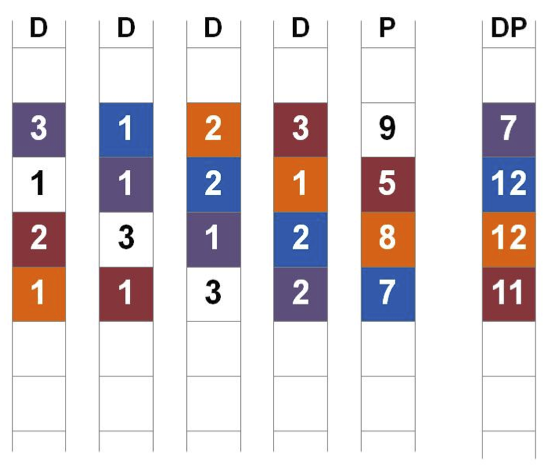
\includegraphics[ keepaspectratio = true]{media/raid-dp.png}
\mycaption{figure}{\label{abb:RAID-DP}NetApp RAID-DP doppelte Parität\cite{White2010}}
\end{center}


Als weiteren Schutzmassnahme vor Datenverluste, empfiehlt NetApp den Einsatz von Spare-Festplatten. Durch den Einsatz von Spare-Festplatten kann die Wiederherstellungszeit MTTR verkleinert werden, da die Wiederherstellung automatisch starten kann. Die Anzahl an Spare-Festplatten ist abhängig von der Anzahl Festplatten und Enclosure.

Die Datenverfügbarkeit kann mittels weiteren NetApp und der Snapmirror Funktion weiter erhöht werden. Dabei werden alle Änderungen an den Daten auf an eine weitere NetApp Synchronisiert. 

NetApp Speichert die Daten auf die Disk in 4 Kilo Byte Blocks. Zu jeden 4 Kilo Byte Block berechnet NetApp eine Prüfsumme und speichert diese in die Block Metadaten. Wenn der Block zu einen späteren Zeitpunkt wieder gelesen ist, berechnet die NetApp die Prüfsumme erneut und vergleicht diese mit der Gespeicherten Prüfsumme. Wenn die Prüfsumme nicht übereinstimmt, wird der Block mittels den Paritäts-Daten neu geschrieben, erneut gelesen und geprüft. Um die Integrität von Daten zu gewährleisten auf welche über eine langen Zeitraum nicht zugegriffen wird, wie diese zum Beispiel bei Archive Daten der Fall ist, hat NetApp eine konfigurierbare RAID durchkämmen (engl. RAID scrub) Funktion. Die Funktion geht durch alle Daten durch, wodurch die Prüfsumme von allen gespeicherten Daten geprüft wird. Die Funktion kann Zeitgesteuert oder wenn das System im Leerlauf befindet. \cite{Sundaram2006}

Zu beachten ist, dass die Prüfsumme auf dem Block nur auf der Speicherebene Wirkung hat. Fehler die in einer höheren Ebene stattfindet, wie zum Beispiel beim Einsatz von iSCSI zusammen mit einen Dateisystem, könnte bereits einen Fehler im Dateisystem durch einen Software Fehler oder Memory Fehler statt finden. 

NetApp bietet mehre Möglichkeiten eine Sicherungskopie der Daten herzustellen. Beim Einsatz von NFS oder iSCSI können die Daten über die Web-Servern mit einer Handels üblichen Sicherungs-Software gesichert werden. Bei NFS wird dazu die angefügten NFS Freigaben gesichert, bei iSCSI werden die Daten wie bei allen anderen Dateisystemen gesichert. Zubeachten ist jedoch, bei diesen verfahren, dass die Daten von der NetApp über den Server transferiert werden müssen, und dadurch der Web-Server mit dem Sicherungslast belastet wird. Neben der Sicherung der NetApp über den Server lässt sich die NetApp auch direkt sichern, dabei gibt es zwei Verfahren, mittels  Network Data Management Protocol (kurz NDMP) oder Mittels Snapshots. 

NDMP ist eines von NetApp mitentwickeltes Protokoll, welches für die Sicherung von NAS Geräte entwickelt wurde. Das Problem bei NAS Geräte ist, dass auf Ihnen ein dezidierte Betriebsystem läuft auf welche keine Installation eines Sicherungs-Agenten erlaubt, aus diesen Grund wurde das NDMP Protokoll entwickelt um eine allgemeines Agenten-Loses Sicherungsverfahren für NAS Geräte zu ermöglichen. NDMP wurde dem IETF im Jahr 2000 von der NDMP Initianden als Entwurf eingereicht, bis anhin ist jedoch noch kein RFC für NDMP Standardisiert. Trotzdem wird es von vielen NAS-Geräte- und Sicherungs-Software- Herstellern unterstützt. Eine Liste mit Sicherungs-Software Produkten, welche das NDMP Verfahren unterstützen gibt es auf der Webseite der NDMP Initianden\footnote{\url{http://www.ndmp.org/products/index.shtml#backup}} zu finden. \cite{NDMP.orga}\cite{NDMP.org}

Beim Snapshots Sicherungsverfahren werden zeitbezogene Sicherung des Dateisystem  erstellt. Bei den Snapshots wird nicht eine eigentliche Kopie der Daten bzw. Blöcke erstellt sondern die Referenz auf die Blöcke gespeichert. Wird nach dem erstellen eines Snapshots ein Block geändert wird die Änderung nicht im Original Block vorgenommen sondern in einen neuen Block und diesen Referenziert. Dadurch benötigt ein Snapshot minimalen Speicher, zudem lassen sich die Snapshots und damit die Sicherung in Sekunden erstellen unabhängig von der Anzahl Dateien oder der Verwendete Speicherkapazität. Durch den Einsatz von zwei NetApp Systemen und der SnapMirror Funktion kann, das ganze Dateisystem bzw. Volume inklusive aller Snapshots auf der zweiten NetApp gesichert werden. Die Sicherung mit Snapshots hat bei grossen Datenmengen entscheidende Vorteile, die Sicherung benötigt minimalen Speicherplatz, die Sicherung und Wiederherstellung ist innert Sekunden erstellt bzw. wiederhergestellt. Nachteile sind, dass der Speicherplatz mit der Sicherung bzw. Snapshots geteilt werden muss und das löschen der Daten zusätzlichen Speicherplatz verbraucht.

%Sicherheit NFS IPSEC, intern



\subsection{\ref{Al-4}: OpenStack Objekt Storage}
OpenStack Object Storage ist eine Quelloffene frei verfügbare Verteilter Speicherlösung. OpenStack Object Storage selbst ist kein Dateisystem sondern eher eine Speicher Cluster, welche primär für die Speicherung von Virtual Maschine Images, Bilder, E-Mail und Sicherungskopien vorgesehen ist. Für einen OpenStack Cluster kommen vergleichbar mit dem Google Filesystem, kosten günstige Konventionelle Computer Hardware zum Einsatz. 


\paragraph{Verfügbarkeit}
OpenStack Object Storage wurde so konzipiert das einen Ausfall einer Hardware Komponente, der weiter Betrieb weiter aufrecht erhalten werden kann ohne dabei einen Datenverlust oder die Verfügbarkeit des System zu gefährden. Die Daten bzw. Objekte werden Redundant auf mehren Zonen gespeichert. Zonen sind Gruppierungen von Servern. Die Anzahl redundanten Replikate für eine Objekt kann konfiguriert werden, gewöhnlich werden drei Kopien verwendet.

Für die Architekt wird von Joe Arnolds CEO bei SwiftStack bei dreifacher Redundanz, die Implementierung von 5 Zone empfohlen. OpenStack Object Storage, speichert die Redundante Objekte jeweils in einer separaten Zonen. Eine Zone kann bei kleinen Implementationen auch nur aus Gruppen von Festplatten bestehen, also innerhalb eines einzigen Server existieren, es wird aber empfohlen eine Zone auf Hierarchie von Server-Gruppen zu implementieren. Das bedeutet jede Redundante Kopie auf einen eigenen Server gespeichert. \cite{Arnold} 

Zusätzlich zu den Speicherserver benötigt es noch zwei oder mehrere Proxy Server um die hohe Verfügbarkeit zu gewährleisten. Die Proxy Server, werden bei Rackspace mit  10 Gb Ethernet an den Netzwerk-Switch angeschlossen werden. \cite{OpenStack2011}

Möchte man den Speicher Standort übergreifend betreiben, ist es erforderlich, dass pro Standort nicht mehr als $(Redundanz -1)$ Zonen betrieben werden, da ansonsten die Gefahr besteht das alle Replikate am gleichen Standort gespeichert werden.

\paragraph*{Speicherkapazität}
Der OpenStack Object Storage Cluster lässt sich im laufenden Betreib ohne Unterbruch, vergrössern. In der Regeln können auch Software Update und Patches ohne Unterbruch des Clusters eingespielt werden, wenn darauf geachtet wird nie mehr als eine Zone gleichzeitig zu aktualisieren.

Grundsätzlich ist Anzahl an Speicherbaren Objekten nicht begrenzt. Der Container Server von OpenStack Object Storage, welcher primärer Aufgabe ist die Auflistung der gespeicherten Objekten in einen Container zu handhaben, speichert die Informationen welche Objekte im Container befinden pro Container in eine SQLite Datenbank. Die Performance der Datenbank, welche mit der Anzahl Einträge abnimmt, kann sich zum Limitierenden Faktor entwickeln wie viele Objekte in einen Container gespeichert werden können. Der Performance Einbruch kann, je nach Leistung der Hardware und die generelle Last auf dem Cluster, bei einer Million Objekte pro Container eintreten. Es können jedoch pro Account mehre Container erstellt werden, wodurch sich das Problem mit der Limitierung durch Datenbank entschärfen lässt. Zu beachten ist hier jedoch, das pro Account ebenfalls eine SQLite Datenbank geführt wird mit allen Container und hier die selben Limitierung zum tragen kommt. \cite{OpenStack2012}\cite{A2011}

\paragraph*{Datenzugriff}
Der Zugriff auf die gespeicherten Objekten erfolgt vergleichbar wie bei Amazon S3 über ein API. Das API verwendet für den Zugriff das Standard HTTP Request. Mehre Speicherlösung Hersteller haben angekündigt, das Swift API ebenfalls für den Zugriff auf Ihren Speicher unterstützen zu wollen. Glusterfs ebenfalls eine Verteile Speicherlösung, bietet in Ihrer Entwickler Version bereits die Unterstützung für Swift an. Applikationen welche, das Swift API unterstützen können Ihren Speicherlösung zukünftig einfacher austauschen ohne dabei die Applikation anpassen zu müssen. Neben den Zugriff mit dem Swift API, bietet OpenStack eine Amazon S3 kompatibles API an. Der Zugriff über POSIX IO auf den Speicher ist nicht möglich.

Der Zugriff auf den Speicher erfolgt über einen Proxy welche, den Speicherort des Objektes prüft und die Anfrage weiterleitet. Pro OpenStack Object Storage Cluster können mehre Proxy eingesetzt werden. Mit Hilfe eines Load Balancers (Last Verteiler) können die Anfragen über die vorhanden Proxy verteilt werden.

Die Maximale Upload Grösse beträgt 5 GB, die Download Grösse selber ist jedoch unbeschränkt. Wenn ein Objekt welches grösser als 5 GB hochgeladen wird, wird das Objekt in Teilen hochgeladen und gespeichert, die Abfrage auf das Objekte erfolgt jedoch wie bei einen ganzen Objekt, es müssen also keine Teile durch das API Adressiert werden. \cite{OpenStack2012a}


\paragraph*{Datenschutz}
OpenStack Object Storage stellt die Datenintegrität beim Speichern von Objekten in den Speicher und beim auslesen der Daten sicher. Somit ist gewährleistet, dass die Daten im Original gespeichert werden und bei der Speicherung kein Datenverlust entsteht. Die Selbstheilung von korrupten Objekten, stellt OpenStack Objekt Storage mit dem Auditors Dienst sicher. Der Auditors Dienst läuft auf jeden Server und prüft dort die Integrität von Objekten, wenn ein korruptes Objekt festgestellt wird, wird die Datei unter Quarantäne gestellt und durch ein korrektes reblikations Objekt ersetzt.
Um die Last die durch den Auditors möglichst gering zu halten, kann die Anzahl Objekte oder die Anzahl Bits die pro Sekunde geprüft werden konfiguriert werden. \cite{OpenStack2012}

OpenStack Objekt Storage bietet neben der Redundanz der Objekte keine Möglichkeit, die Daten zu Sichern. Dadurch ist keine Versionierung der Objekte möglich. Zwar lässt sich die Cluster Nodes mit einen konventionellen Sicherungssoftware direkt sichern, jedoch wurde sich nur der gesamte Cluster wiederherstellen und nicht einzelne Objekte. Zudem wäre die Speicherkapazität pro Sicherung, so gross wie es für die redundante Speicherung der Objekte Speicherkapazität benötigt wird. \cite{AndyBrezinsky2011}


Die Sicherheit der Daten wird mit sogenannten Accounts Sichergestellt, dass heist das ein Account nur auf seine gespeicherten Objekten zugreifen kann. Die Daten werden auf dem OpenStack Cluster Unverschlüsselt in Binären form gespeichert. Durch die Verteilung der Daten müsste jedoch eine Angreifer Zugriff auf alle Cluster Node erlangen um an alle Daten eines Account zu gelangen.

\paragraph*{Technologie}
OpenStack Objekt Storage wurde von der Firma RackSpace unter dem Code Name Swift entwickelt. Zusammen mit National Aeronautics and Space Administration (kurz. NASA) hat RackSpace die Softwareprojekt-Gemeinschaft OpenStack gegründet und Swift zusammen mit den Cloud Lösungen Nova für die Verwaltung von Virutellen Maschinen und Glace für die Verwaltung von Image als Quelloffene Software veröffentlicht. Die OpenStack Gemeinschaft ist in Vergleich zu anderen Quelloffenen Gemeinschaften noch eine relative jung Gemeinschaft, es gelangt Ihr dennoch neben den beiden Gründer Unternehmen, weiter bedeutende Unternehmen aus der Informatik Branche, wie Hewlett Packard, Dell, Citrix, Intel, AMD, NetApp und weitere zu gewinnen. Eine vollständige Liste aller Unterstützende  Unternehmen ist unter \url{http://openstack.org/community/companies/} zu finden. Die Aktivität auf der Projekt Seite von OpenStack Object Storage, lässt erkennen, dass die Entwicklung aktive vorangetrieben wird und viele Beiträge zur neuen Funktionen oder Verbesserungen von Anwender und Entwickler bei gesteuert werden. \cite{Ohloh2012}

Die Internet-Recherche auf OpenStack spezialisierte Firmen mit Standort Schweiz ergaben keine Ergebnisse. Einige
Gemäss Internet Recherchen gibt es noch keine spezialisierte Firma für OpenStack Lösungen. Einige wenige Experten für OpenStack mit Domizil in der Schweiz konnten über die Profile bei LinkedIn einen Soziales Netzwerk für Geschäft gefunden werden. 

Die Verwaltung des Speichers bietet OpenStack ein Kommandozeilen Tools an. Ein Web-GUI für Objekt Storage von OpenStack gibt es nicht. Die Firma SwiftStack bietet hierfür jedoch Kostenpflichtige Lösungen an. Die Überwachung des Speichers, zum Beispiel die Verfügbarkeit einzelner Cluster Nodes, muss jedoch mit zusätzlichen Fremdlösungen erfolgen. 

\subsubsection{Kosten}
Grundsätzlich unterscheidet sich die Kosten für die beiden Szenario nur in der Anzahl Server, den Verwendeten Server Typen, in der Anzahl Festplatten und den benötigten Rack Platz. Die restlichen Faktoren sind für beide Szenerien die selben und werden in diesen Abschnitt behandelt.

Um die Kosten der Rechenzentrumskosten möglichst tief zu halten, welche pro Rack verrechnet werden, soll möglichst viel Speicherkapazität in eine Rackeinheit gepackt werden. Dass bedeutet, dass die Richtigen Server für die Anzahl zur Verfügung gestellten Speicherkapazität verwendet werden soll.

Um die Preise für die Festplatten möglichst tief zu halten werden diese separate beschaffen. Als Festplatte soll eine SATA-3 3.5 Zoll 3 Terabyte Festplatte eingesetzt werden, diese entspricht 2.728 Tebibyte. Die Kosten für Festplatten sind stark Marktabhängig, für die Arbeit wird deshalb der einfachhalber mit ca. 300 CHF pro Festplatte gerechnet.

Für beide Szenerien werden die gleichen Proxy-Server verwendet. Als Proxy Server wurden die Transtec Server-Systeme "'Lynx CALLEO Application Server 2260S'" ausgewählt. Die Proxy Server stammen von selben Hersteller wie die in den Szenerien aufgeführten Datenserver, diese hat den Vorteil, dass nur ein Ansprechpartner für die Server Hardware gibt. Es ist jedoch kein muss Kriterium und kann bei bedarf auch durch eine besseres Angebot eines anderen Hersteller ersetzt werden. Die Proxy sind mit einen Intel Xeon Prozessor E5-2665 mit 64 Gigabyte Hauptspeicher ausgerüstet. Die Server haben eine Rack-Höheneinheit von je 2 Einheiten. Wie bei den Datenserver wurde ein 365 mal 24 Stunden vor Ort Service ausgewählt. Der Preis pro Server beträgt 9'954 CHF.

Neben der Server Infrastruktur sind noch zwei Netzwerk-Switches notwendig. Der Dell PowerConnect 8024 bietet 24 Port mit 10GbE. Die Switch haben eine Rack-Höheneinheit von je 1 Einheiten und benötigen gemäss Hersteller maximal 237,77 Watt. Dell gewährt einen 3 Jahres Support für den Switch. Der Preis pro Switch beträgt 14'732 CHF.

Als Rechenzentrum Betreiber wurde Nine Internet Solution ausgewählt. Nine Betreibt seine Rechenzentrum in Zürich und ist auf die Hosting Spezialisiert. Mit seinen Rechenzentrum Standort in der Stadt Zürich, befindet sich Nine Geographisch in der Nähe des Auftraggeber. Die Anfahrtszeit und Anfahrtsweg kann so für den Auftraggeber kurz gehalten werden. Die Verschiedenen Rack Produkte welche Nine anbietet, unterscheiden sich von der Anzahl beinhalteten Rack-Höheneinheiten und deren beinhalteten Watt Leistung. In den Produkten ist zusätzlich die Anbindung ans  Internet Anbindung mit 100 Mbps beinhaltet. Bei Zusätzlichen Watt bedarf, bietet Nine die Möglichkeit die Zusätliche Watt in 500 Pakete zu 165 CHF pro Monat an.

Für den den Betrieb der Speicherinfrastruktur wird mit einer Mann Stelle gerechnet. Organisatorisch kann diese auch auf mehre Prozentual Stellen aufgeteilt werden, somit ist auch der Betreib während Ferien Abwesenheit geregelt. Pro Monat wird mit Personal Kosten von 15'000 CHF gerechnet.


\paragraph*{Kosten Szenario-1}

Für die dreifache Redundanz sind für die aus der Soll-Analyse bestimmten 306 Tebibyte gemäss \refeqlb{eqn:SpeicherkapazitätS1} 918 Tebibyte an Speicherkapazität notwendig.

\begin{equation}
\mbox{Speicherkapazität}_{Redundanz} = 306  \mathrm{\ TiB} * 3 \mbox{\ Redundanz} =  918 \mathrm{\ TiB}
\label{eqn:SpeicherkapazitätS1}
\end{equation}


Als Server System wurde der Transtec Lynx CALLEO Application Server 1260 gewählt. Der Server basiert auf Server Hardware des Herstellers  SuperMicro. Der Server benötigt 1 Rack-Höcheneinheiten Rack platz und bieten Platz für den Einbau von 4 3.5 Zoll Festplatten, welche auch während des Betriebs ausgetauscht werden können. Als Prozessoreinheit kommen ein Intel Xeon Prozessor E5-2620 zum Einsatz, zudem verfügt der Server über 32 Gigabyte Hauptspeicher. Der Server wurde mit einen 3 Jahres, 24 Stunden, 365 Tage im Jahr Vor-Ort Service ausgestattet. Somit ist sichergestellt, das im Störungsfall der Unterbruch möglichst gering gehalten werden kann. Der Preis pro Server beträgt ohne Festplatten 1'260 CHF.


Ein Server welche voll Ausgerüstet mit Festplatten, weist gemäss der  \refeqlb{eqn:SpeicherkapazitätServerS1} eine Speicherkapazität von 10,912 Tebibyte aus. Damit sind in Anbetracht der notwendigen Speicherkapazität von 48,3 Tebibyte und der 5 Zonen insgesamt 5 Server notwendig (siehe \refeqlb{eqn:AnzahlServerS1}). Für die Erreichung der Speicherkapazität von 48,3 Tebibyte bei gleich ausgerüsteten Server sind jedoch insgesamt nur 20 Festplatten notwendig.

\begin{equation}
\mbox{Speicherkapazität}_{Server} = 2,728 \mathrm{\ TiB} * 4 \mbox{\ Einschub} =  10,912 \mathrm{\ TiB}
\label{eqn:SpeicherkapazitätServerS1}
\end{equation}

\begin{equation}
\mbox{Anzahl Server} = \frac{48,3 \mathrm{\ TiB}}{10,912 \mathrm{\ TiB}} \approx  5 \mbox{\ (Auf 5 Zonen gerundet)}
\label{eqn:AnzahlServerS1}
\end{equation}

\begin{equation}
\mbox{Anzahl Festplatten} = \frac{48,3 \mathrm{\ TiB}}{2,728 \mathrm{\ TiB}} \approx  20 \mbox{\ (Auf 5 Server gerundet)}
\label{eqn:AnzahlServerS1}
\end{equation}

Gemäss \refeqlb{eqn:AnzahlRackS1} wird ein viertel Rack für den Einbau aller Komponenten. Der Benötigte Rack Platz entspricht den Quarter Rack Angebot von Nine, welches 11 Rack-Höheneinheiten platz bietet. Der Preis pro Rack beträgt 450 CHF pro Monat, plus 650 CHF für die einmalige Einrichtung des Racks durch Nine.
Für die Berechnung der Gesamt Watt Leistung welcher der Server im Betrieb benötigt, fehlen die Angaben des Hersteller. Aus diesen Grund wird angenommen, dass der Daten-Server ca. 300 Watt und der Proxy-Server 500 Watt bezieht. Mit diesen Annahmen benötigt es gemäss  \refeqlb{eqn:AnzahlWattPaketeS1}, den 500 Watt welche im Rack beinhaltet sind, zusätzliche 5 Pakete a 500 Watt pro Monat.

\begin{equation}
\mbox{Anzahl Racks} = \frac{5 * 1 \mathrm{\ U} + 2 * 2 \mathrm{\ U} + 2 * 2 \mathrm{\ U}}{11\mathrm{\ U}} \approx  1 \mbox{\ (Auf viertel Rack gerundet)}
\label{eqn:AnzahlRackS1}
\end{equation}

\begin{equation}
\mbox{Anzahl 500 \mathrm{W} Pakete} = \frac{5 * 300 \mathrm{\ W} + 2 * 500 \mathrm{\ W} +2 * 237,77 \mathrm{\ W} - 2000 \mathrm{\ W} }{500\mathrm{\ W}} \approx  5
\label{eqn:AnzahlWattPaketeS1}
\end{equation}

Wie aus der \reftab{tab:KostenOpenStackS1} ersichtlich ist, betragen die Gesamtkosten 653'646.50 CHF.


\begin{table}[htbp]
\caption{Kosten OpenStack S1}
\begin{small}
\begin{tabular}{|l|r|r|r|}
\hline
\textbf{Beschreibung} & \multicolumn{1}{l|}{\textbf{Kosten pro Stk/M.}} & \multicolumn{1}{l|}{\textbf{Anzahl}} & \multicolumn{1}{l|}{\textbf{Total}} \\ \hline
  \multicolumn{ 4}{c}{} \\  \hline
\multicolumn{ 4}{|c|}{\textbf{Investitionskosten}} \\ \hline
Dell PowerConnect 8024 & CHF 14'732.00 & 2 & CHF 29'464.00 \\ \hline
Lynx CALLEO App. Server 1260 & CHF 5'451.50 & 2 & CHF 10'903.00 \\ \hline
Lynx CALLEO App. Server 1260 & CHF 2'831.30 & 5 & CHF 14'156.50 \\ \hline
Festplatte 3,5 3 TB & CHF 300.00 & 20 & CHF 6'000.00 \\ \hline
Rack Einrichtung & CHF 650.00 & 1 & CHF 650.00 \\ \hline \hline
  \multicolumn{ 3}{r|}{\textbf{Total:}}  & \textbf{CHF 61'173.50} \\ 
  \cline{4-4}
\multicolumn{ 4}{c}{} \\   \hline
\multicolumn{ 4}{|c|}{\textbf{Fortlaufende Kosten}} \\ \hline
Dell Service  & CHF 0.00 & 2 & CHF 0.00 \\ \hline
Transtec Service (Server 1260) & CHF 26.08 & 2 & CHF 52.17 \\ \hline
Transtec Service (Server 1260) & CHF 26.08 & 5 & CHF 130.42 \\ \hline
Rackkosten 11 U (500 W) & CHF 450.00 & 1 & CHF 450.00 \\ \hline
Strom 500 W & CHF 165.00 & 5 & CHF 825.00 \\ \hline
Personal & CHF 15'000.00 & 1 & CHF 15'000.00 \\ \hline \hline
  \multicolumn{ 3}{r|}{\textbf{Total pro Monat:}} & CHF 16'457.58 \\
\cline{4-4}
  \multicolumn{ 3}{r|}{\textbf{Total 36 Monate:}} & \textbf{CHF 592'473.00} \\ \cline{4-4}
  \multicolumn{ 4}{c}{} \\  \cline{4-4}
  \multicolumn{ 3}{r|}{\textbf{Total Gesamt:}} & \textbf{CHF 653'646.50} \\ \cline{4-4}
\end{tabular}
\end{small}
\label{KostenOpenStackS1}
\end{table}



\subsubsection{Kosten Szenario-2}

Für die dreifache Redundanz sind für die aus der Soll-Analyse bestimmten 306 Tebibyte gemäss \refeqlb{eqn:SpeicherkapazitätS2} 918 Tebibyte an Speicherkapazität notwendig.

\begin{equation}
\mbox{Speicherkapazität}_{Redundanz} = 306  \mathrm{\ TiB} * 3 \mbox{\ Redundanz} =  918 \mathrm{\ TiB}
\label{eqn:SpeicherkapazitätS2}
\end{equation}


Als Server System wurde der Transtec Lynx CALLEO Application Server 4260 gewählt. Der Server basiert auf Server Hardware des Herstellers  SuperMicro, welche gemäss eigenen Recherchen auch bei anderen OpenStack Lösungen verwendet wird. Der Server benötigt 4 Rack-Höcheneinheiten Rack platz und bieten Platz für den Einbau von 36 3.5 Zoll Festplatten, welche auch während des Betriebs ausgetauscht werden können. Als Prozessoreinheit kommen zwei Intel Xeon Prozessor E5-2620 zum Einsatz, zudem verfügt der Server über 64 Gigabyte Hauptspeicher. Der Server wurde mit einen 3 Jahres, 24 Stunden, 365 Tage im Jahr Vor-Ort Service ausgestattet. Somit ist sichergestellt, das im Störungsfall der Unterbruch möglichst gering gehalten werden kann. Der Preis pro Server beträgt ohne Festplatten 8'672 CHF.


Ein Server welche voll Ausgerüstet mit Festplatten, weist gemäss der  \refeqlb{eqn:SpeicherkapazitätServerS2} eine Speicherkapazität von 98.208 Tebibyte aus. Damit sind in Anbetracht der notwendigen Speicherkapazität von 918 Tebibyte und der 5 Zonen insgesamt 10 Server notwendig (siehe \refeqlb{eqn:AnzahlServerS2}). Für die Erreichung der Speicherkapazität von 918 Tebibyte bei gleich ausgerüsteten Server sind jedoch insgesamt nur 340 Festplatten notwendig, dass heisst pro Server sind 34 Einschub mit Festplatten belegt. Sie könnten also bei Bedarf noch weiter aufgerüstet werden.

\begin{equation}
\mbox{Speicherkapazität}_{Server} = 2,728 \mathrm{\ TiB} * 36 \mbox{\ Einschub} =  98.208 \mathrm{\ TiB}
\label{eqn:SpeicherkapazitätServerS2}
\end{equation}

\begin{equation}
\mbox{Anzahl Server} = \frac{918 \mathrm{\ TiB}}{98.208 \mathrm{\ TiB}} \approx  10 \mbox{\ (Auf 5 Zonen gerundet)}
\label{eqn:AnzahlServerS2}
\end{equation}

\begin{equation}
\mbox{Anzahl Festplatten} = \frac{918 \mathrm{\ TiB}}{2,728 \mathrm{\ TiB}} \approx  340 \mbox{\ (Auf 10 Server gerundet)}
\label{eqn:AnzahlServerS2}
\end{equation}

Gemäss \refeqlb{eqn:AnzahlRackS2} wird ein ganzes Rack für den Einbau aller Komponenten. Der Benötigte Rack Platz entspricht den Full Rack Angebot von Nine, welches 47 Rack-Höheneinheiten platz bietet. Der Preis pro Rack beträgt 1450 CHF pro Monat, plus 1500 CHF für die einmalige Einrichtung des Racks durch Nine.
Für die Berechnung der Gesamt Watt Leistung welcher der Server im Betrieb benötigt, fehlen die Angaben des Hersteller. Aus diesen Grund wird angenommen, dass der Daten-Server ca. 700 Watt und der Proxy-Server 500 Watt bezieht. Mit diesen Annahmen benötigt es gemäss  \refeqlb{eqn:AnzahlWattPaketeS2}, den 2000 Watt welche im Rack beinhaltet sind, zusätliche 13 Pakete a 500 Watt pro Monat.

\begin{equation}
\mbox{Anzahl Racks} = \frac{10 * 4 \mathrm{\ U} + 2 * 2 \mathrm{\ U} + 2 * 2 \mathrm{\ U}}{47\mathrm{\ U}} \approx  1 \mbox{\ (Auf ganze Rack gerundet)}
\label{eqn:AnzahlRackS2}
\end{equation}

\begin{equation}
\mbox{Anzahl 500 \mathrm{W} Pakete} = \frac{10 * 700 \mathrm{\ W} + 2 * 500 \mathrm{\ W} +2 * 237,77 \mathrm{\ W} - 2000 \mathrm{\ W} }{500\mathrm{\ W}} \approx  13
\label{eqn:AnzahlWattPaketeS2}
\end{equation}

Wie aus der \reftab{tab:KostenOpenStackS1} ersichtlich ist, betragen die Gesamtkosten 893'965 CHF.

\begin{table}[htbp]
\caption{Kosten OpenStack}
\begin{small}
\begin{tabular}{|l|r|r|r|}
\hline
\textbf{Beschreibung} & \multicolumn{1}{l|}{\textbf{Kosten pro Stk/M.}} & \multicolumn{1}{l|}{\textbf{Anzahl}} & \multicolumn{1}{l|}{\textbf{Total}} \\ \hline
  \multicolumn{ 4}{c}{} \\  \hline
\multicolumn{ 4}{|c|}{\textbf{Investitionskosten}} \\ \hline
Dell PowerConnect 8024 & CHF 14'732.00 & 2 & CHF 29'464.00 \\ \hline
Lynx CALLEO App. Server 1260 & CHF 5'451.50 & 2 & CHF 10'903.00 \\ \hline
Lynx CALLEO App. Server 4260H & CHF 6'111.00 & 10 & CHF 61'110.00 \\ \hline
Festplatte 3,5 3 TB & CHF 300.00 & 340 & CHF 102'000.00 \\ \hline \hline
  \multicolumn{ 3}{r|}{\textbf{Total:}} & \textbf{CHF 203'477.00} \\ \cline{4-4}
\multicolumn{ 4}{c}{} \\   \hline
\multicolumn{ 4}{|c|}{\textbf{Fortlaufende Kosten}} \\ \hline
Dell Service  & CHF 0.00 & 2 & CHF 0.00 \\ \hline
Transtec Service (Server 1260) & CHF 26.08 & 2 & CHF 52.17 \\ \hline
Transtec Service (Server 4260H) & CHF 53.31 & 10 & CHF 533.06 \\ \hline
 Rackkosten 47 U (2000 W) & CHF 1'450.00 & 1 & CHF 1'450.00 \\ \hline
Strom 500 W  & CHF 165.00 & 13 & CHF 2'145.00 \\ \hline
Personal & CHF 15'000.00 & 1 & CHF 15'000.00 \\ \hline \hline
  \multicolumn{ 3}{r|}{\textbf{Total pro Monat:}} & CHF 19'180.22 \\ \cline{4-4}
  \multicolumn{ 3}{r|}{\textbf{Total 36 Monate:}} & \textbf{CHF 690'488.00} \\ \cline{4-4}
  \multicolumn{ 4}{c}{} \\  \cline{4-4}
  \multicolumn{ 3}{r|}{\textbf{Total Gesamt:}} & \textbf{CHF 893'965.00} \\ \cline{4-4}
\end{tabular}
\end{small}
\label{tab:KostenOpenStackS2}
\end{table}


\subsection{\ref{Al-5}: Amazon S3}
Amazon zählt zu den Grössten, wenn nicht der grösste Online Speicheranbieter weltweit. Genaue Anzahlen über die Anzahl Kunden und Speicherkapazität veröffentlich Amazon nicht. Seit 2006 bietet Amazon Ihren Kunden unter den Produktname S3, einen Online Speicher an. Die genaueren Technischen Eigenschaften und Architektur des Online Speicher ist bis anhin von Amazon nicht veröffentlicht worden. Nach eigenen Angaben von Amazon basiert die Dienstleistung auf gewöhnlichen Computer Hardware.






Bei Online Speicher wie Amazon S3, kann der Kunde gleich nach Anmeldung an den Dienst, die Speicherressourcen verwenden. Es fallen also keine Installation von für
die Speicherinfrastruktur an. 

\paragraph*{Verfügbarkeit}
Amazon S3 Speichert die Daten auf mehren Geräten in Verschiedenen Rechenzentren in der selben Region ab. Bei speichern werden die Daten Synchron in Verschiedene Rechenzentren gespeichert bevor die Speicherung als erfolgreich gemeldet ist, damit ist sicher gestellt, dass die Daten von beginn weg Redundant gespeichert sind. Mit diesen Massnahmen gewährleistet Amazon gemäss Dienstgütevereinbarung eine Zuverlässigkeit von 99.999999999\%. Bei bedarf kann die Zuverlässigkeit für Daten welche wenig Schutz benötigen, wie zum Beispiel Thumbnails von Bilder, mit einer geringeren Zuverlässigkeit von 99.99\% zu einen günstigeren Preis gespeichert werden. \cite{Amazon2007}

Durch die Redundante Speicherung der Daten auf mehre Geräten gewährleistet Amazone gemäss Dienstgütevereinbarung von 99.99\% pro Monat

\paragraph*{Datenzugriff}
Der Zugriff auf die Daten findet über eine API oder über die Verwaltungskonsole von Amazon statt. Für den Zugriff mit einen API bietet Amazon ein \gls{REST} und ein \gls{SOAP} Schnittstelle an. Der \gls{REST} Zugriff findet über HTTP statt, dabei werden Standard HTTP requests verwendet. Für den Zugriff kann auch einen gewöhnlichen Web-Browser verwendet werden solange die Objekte Öffentlich sind.

Einen Offiziellen POSIX IO Zugriff von Amazon steht nicht zur Verfügung, es existiert jedoch eine Quelloffenes Projekt Namens s3fs\footnote{\url{https://code.google.com/p/s3fs/}} welche es ermöglicht eine Amazon S3 Speicher unter Linux zu mounten. \cite{S3fs}

Da die Infrastruktur von Amazon S3 nicht bekannt ist, können keine detailierte Angaben wie Amazon die Skalierung der Datenzugriffe handhabt. Es kann jedoch von einen hochskalierbaren System ausgegangen werden, da Amazon die Zugriffe von tausenden von Kunden gleichzeitig handhaben muss.

Amazon S3 unterstützt das Lesen und Schreiben von mehren Systemen. Beim Lesen einen Objekts welche von mehren Systemen Zugegriffen wird und beschrieben, stellt Amazon S3 die Lese konsistent sicher. \cite{Amazon2012a}

Für das Einlesen von Grossen Datenmengen bietet Amazon einen kostenpflichtigen Import/Export Dienstleistung an. Bei dieser Dienstleistung sendet der Kunde die Daten gespeichert auf  einen tragbares Speichergeräte an Amazon, welches die Daten direkt in Ihre Cloud ohne Umwege über das Internet einliesst.

Die API von Amazon ist gut Dokumentiert, weshalb für einen erfahrenen Entwickler die Anbindung der Web-Applikation an Amazon S3 umsetzbar sein sollte.

\paragraph*{Speicherkapazität}
Für die Skalierung der Speicherkapazität kümmert sich Amazon.

Im Amazon S3 können eine unbegrenzte Zahl von Objekten gespeichert werden, welche eine Speichergrösse von 1 Byte bis zu 5 Terrabyte haben können, wobei aber in einen PUT maximal 5 Gigabyte hochgeladen werden können. Für das Hochladen von Grösseren Objekten, muss die Multipart Funktion verwendet werden, welche das Objekte in mehren Teilen hochladet.\cite{Amazon2012b}

\paragraph*{Datenschutz}
Die Daten können bei Amazon in mehren Regionen gespeichert werden. Zu den verfügbaren Regionen gehören, US Standard, US West (Oregon), US West (Northern California), EU (Ireland), Asia Pacific (Singapore), Asia Pacific (Tokyo), South America (Sao Paulo). Gemäss Amazon verlassen die Gespeicherten Daten eine Region nicht, ausser für die Erfüllung von Gesetzen oder auf Anforderung von Regierung Anweisung. Als US Amerikanisches Unternehmen steht Amazon wegen dem Patrot Act, unter der Pflicht, den USA Behörden Zugang zu Informationen zu gewährleisten auf behördlichen Anforderungen, auch wenn diese Informationen ausserhalb der USA gespeichert sind. Gemäss EU Recht darf jedoch keine gespeicherten Informationen, an dritten Zugänglich gemacht werden oder ausserhalb der EU gespeichert werden, ohne Einverständnis. Bei Microsoft ebenfalls eine Grosser Cloud Anbieter bestätigt diese Annahme, das die Daten nicht vor den Zugriff der USA geschützt sind.\cite{Amazon2012}\cite{Ostler}

Die Integrität der Daten wird mit einer Prüfsumme sichergestellt. Die gespeicherten Daten werden von Amazon regelmässig auf Ihre Integrität geprüft und bei bedarf von einer Integer Kopie der Daten ersetzt. 

Die Daten können Verschlüsselt per SSL Zugegriffen bzw. gespeichert werden, somit ist gewährleistet, das dritte die Daten beim Transport nicht lesen können. Seit 2011 bietet Amazon kostenlos ebenfalls die Verschlüsselung mit AES-256 von Objekten im Speicher an. Dabei wird jedes Objekt mit einen eigenen Schluss ver- und entschlüsselt. Die erzeugten Schlüssel werden mit einen Master-Schlüssel ebenfalls Verschlüsselt und auf den Amazon-Servern gespeichert. Das Schlüsselmanagment bleibt jedoch bei Amazon, weshalb man abhängig von den Massnahmen zum schuzt des Schlusselmanagment die Amazon trifft. Wird diese Kompromittiert oder fällt aus ist der Zugriff auf die Verschlüsselten Daten nicht mehr möglich.\cite{RobertLippert2011}

Die Berechtigung auf gespeicherte Objekte oder Ordner können mit einen Rechte-Management verwaltet werden. Objekte können öffentlich zugänglich gemacht werden oder nur an bestimmte Authentifizierte Benutzer zur Verfügung gestellt werden. Zudem lassen Sich Zugriffe auf Objekte Protokollieren.\cite{Amazon2012b}

Für die Berechtigung und Verwaltung stellt Amazon ein Web-GUI zur Verfügung. Bis auf das eröffnen eines Speichers und die Initial Berechtigung sollten, wahrscheinlich nicht viel mehr Verwaltungsaufgaben anfallen.

Amazon bietet neben der Redundanz der Objekte kein weiteres Sicherungsverfahren an. Beim Herunterladen der Daten fallen für den Transfer weiter Kosten an.

\paragraph*{Technologie}
Der Online Speicher von Amazon S3 gilt als ausgereiftes und etabliertes Produkt im Markt, weshalb davon ausgegangen werden kann, dass die Dienstleistung über die nächsten vier Jahre drübenraus noch bestehen wird und für den Kunden keine Migration notwendig ist. Amazon S3 wird ebenfalls von SmugMug ebenfalls eine Photodienstleister oder andere bekannte Web-Applikationen wie Dropbox verwendet.\cite{SmugMug}\cite{Dropbox2011}

Der Online Speicher Markt ist im Verhältnis zu anderen Speicher Märkte noch relativ jung, Analysten wie Jeff Boles gehen davon aus, dass der Online Speicher Markt in den nächsten Jahren weiter stark wächst. Wie in der Marktstudie beschrieben konnte Amazon seit dem Start des Amazon S3 Produktes die Anzahl gespeicherte Objekte jeweils pro Jahr mehr als verdoppeln (sie dazu \refabb{abb:AnzahlObjekteAmazonS3}). Die Konkurrenz von grossen Anbietern wie Google, Microsoft oder Rackspace nimmt für Amazon bereits zu. Für den Kunden bedeutet diese, dass die Anbieter Ihre Preise noch stärker kalkulieren müssen um ein Konkurrenz fähiges Angebot zu haben. Amazon hat die Preise für S3 Speicher erst kürzlich angepasst.\cite{Boles2011}\cite{Barr2012a}


\subsubsection{Kosten}
Durch den Bezug des Speichersressourcen als Dienstleistung, fallen für den Kunden keine Investitionskosten für die Speicher Infrastruktur an.
Dafür muss in den meisten Fällen, die Applikation für den Zugriff mittels Amazon S3 API vorbereitet werden, wodurch Entwicklungskosten anfallen könnten.

Beim Amazon S3 wird jeweils nur der Effektive verwendete Speicherplatz pro Monat verrechnet, im Preis von Amazon ist jeweils die dreifache Redundanz inbegriffen. Der Speicherplatz Kostet ab 1 Terabyte bis 49 Terabyte \$ 0.110 per Gigiabyte. Ab 49 Terabyte bis 450 Terabyte reduzieren sich die Kosten pro Gigabyte auf \$ 0.095. Anders als beim betrieb seiner eigenen Speicherinfrastruktur muss der Kunden keine zusätzliche Speicherkapazitätsreserven für unvorhergesehenes einrechnen, da Ihm diese bei Bedarf jederzeit von Amazon zur Verfügung gestellt wird, was wiederum die Kosten für den Kunden senkt, da er keine Reserve zu Verfügung stellen muss.

Bei Verwendung von Amazon S3 fallen für den Kunden zudem keine Wartungskosten für den Betrieb der Speicherinfrastruktur an. 

Im vergleich zu betrieb der eignen Speicherinfrastruktur, fallen dem Kunden, stattdessen Kosten für den Transfer und Abfragen der Daten an, welche bei der eignenden Infrastruktur generell durch die Investition in die Infrastruktur beinhaltet ist. So Kostet der Transfer der Daten aus der Amazon S3 Speicher aus, für jedes GB \$ 0.12 bei einen Transfervolumen bis 10 TB.  Für die Abfrage wird unterschieden zwischen Schreibenden und Lesenden Abfragen. Für den Lese Zugriff auf die Daten wird pro 10'000 Abfragen \$ 0.01 und für jede Schreibzugriff pro 1'000 Abfragen\$ 0.01 verrechnet. Gerade diese Kosten sind jedoch schwer vorher zubestimmen und könnten zu Überraschungen sorgen. Grund dafür ist, dass diese jeweils stark von jeweiligen Anzahl Benutzer und deren Benutzerverhalten abhängig sind und diese schwer zu vorhersagen ist.

\paragraph*{Kosten Szenario-1}
Die Kosten für Szenario-1 betragen gemäss Zusammenstellung der\reftab{tab:KostenAmazonS3S1} Total  \$ 42'646.32 das sind zum aktuellen Tageskurs (13 April 2012)  39'10.52 CHF. 


\subsubsection*{Kosten Szenario-2}
Die Kosten für Szenario-1 betragen gemäss Zusammenstellung der \reftab{tab:KostenAmazonS3S2} Total  \$ 493'902.84 das sind zum aktuellen Tageskurs (13 April 2012)  450'637.17 CHF. 

\begin{table}
\caption{Kosten Amazon S3 Szenario-1}
\begin{center}
\begin{tabular}{|l|r|r|r|}
\hline
\multicolumn{1}{|l|}{\textbf{Bezeichnung}} &\multicolumn{1}{|l|}{\textbf{Monat}} & \multicolumn{1}{l|}
{\textbf{Speicherkapazität}} & \multicolumn{1}{l|}{\textbf{Kosten}} \\ \hline
\multicolumn{4}{c}{} \\  \hline
\multicolumn{ 4}{|c|}{\textit{Investitionskosten}} \\ \hline 
- &  &  &    \\ \hline
\multicolumn{3}{r|}{\textbf{Total:}} & CHF 0.00 \\ \cline{4-4}
\multicolumn{4}{c}{} \\  \hline
\multicolumn{ 4}{|c|}{\textit{Fortlaufende Kosten}} \\ \hline
Amazon S3 & 1 & 2,75 &  \$691.82  \\ \hline
Amazon S3 & 2 & 3 &  \$719.98  \\ \hline
Amazon S3 & 3 & 3,25 &  \$748.14  \\ \hline
Amazon S3 & 4 & 3,5 &  \$776.30  \\ \hline
Amazon S3 & 5 & 3,75 &  \$804.46  \\ \hline
Amazon S3 & 6 & 4 &  \$832.62  \\ \hline
Amazon S3 & 7 & 4,25 &  \$860.78  \\ \hline
Amazon S3 & 8 & 4,5 &  \$888.94  \\ \hline
Amazon S3 & 9 & 4,75 &  \$917.10  \\ \hline
Amazon S3 & 10 & 5 &  \$945.26  \\ \hline
Amazon S3 & 11 & 5,25 &  \$973.42  \\ \hline
Amazon S3 & 12 & 5,5 &  \$1'001.58  \\ \hline
Amazon S3 & 13 & 5,75 &  \$1'029.74  \\ \hline
Amazon S3 & 14 & 6 &  \$1'057.90  \\ \hline
Amazon S3 & 15 & 6,25 &  \$1'086.06  \\ \hline
Amazon S3 & 16 & 6,5 &  \$1'114.22  \\ \hline
Amazon S3 & 17 & 6,75 &  \$1'142.38  \\ \hline
Amazon S3 & 18 & 7 &  \$1'170.54  \\ \hline
Amazon S3 & 19 & 7,25 &  \$1'198.70  \\ \hline
Amazon S3 & 20 & 7,5 &  \$1'226.86  \\ \hline
Amazon S3 & 21 & 7,75 &  \$1'255.02  \\ \hline
Amazon S3 & 22 & 8 &  \$1'283.18  \\ \hline
Amazon S3 & 23 & 8,25 &  \$1'311.34  \\ \hline
Amazon S3 & 24 & 8,5 &  \$1'339.50  \\ \hline
Amazon S3 & 25 & 8,75 &  \$1'367.66  \\ \hline
Amazon S3 & 26 & 9 &  \$1'395.82  \\ \hline
Amazon S3 & 27 & 9,25 &  \$1'423.98  \\ \hline
Amazon S3 & 28 & 9,5 &  \$1'452.14  \\ \hline
Amazon S3 & 29 & 9,75 &  \$1'480.30  \\ \hline
Amazon S3 & 30 & 10 &  \$1'508.46  \\ \hline
Amazon S3 & 31 & 10,25 &  \$1'536.62  \\ \hline
Amazon S3 & 32 & 10,5 &  \$1'564.78  \\ \hline
Amazon S3 & 33 & 10,75 &  \$1'592.94  \\ \hline
Amazon S3 & 34 & 11 &  \$1'621.10  \\ \hline
Amazon S3 & 35 & 11,25 &  \$1'649.26  \\ \hline
Amazon S3 & 36 & 11,5 &  \$1'677.42  \\ \hline
\multicolumn{3}{r|}{\textbf{Total:}} & \textbf{\$ 42'646.32} \\ \cline{4-4}
\multicolumn{4}{c}{} \\  \cline{4-4}
\multicolumn{3}{r|}{\textbf{Total Gesamt:}} & \textbf{ \$ 42'646.32} \\ \cline{4-4}
\end{tabular}
\end{center}
\label{tab:KostenAmazonS3S1}
\end{table}

\begin{table}
\caption{Kosten Amazon S3 Szenario-2}
\begin{center}
\begin{tabular}{|l|r|r|r|}
\hline
\multicolumn{1}{|l|}{\textbf{Bezeichnung}} &\multicolumn{1}{|l|}{\textbf{Monat}} & \multicolumn{1}{l|}
{\textbf{Speicherkapazität}} & \multicolumn{1}{l|}{\textbf{Kosten}} \\ \hline
\multicolumn{4}{c}{} \\  \hline
\multicolumn{ 4}{|c|}{\textit{Investitionskosten}} \\ \hline 
- &  &  &    \\ \hline
\multicolumn{3}{r|}{\textbf{Total:}} & CHF 0.00 \\ \cline{4-4}
\multicolumn{4}{c}{} \\  \hline
\multicolumn{ 4}{|c|}{\textit{Fortlaufende Kosten}} \\ \hline
Amazon S3 & 1 & 8.5 &  \$2'937.87  \\ \hline
Amazon S3 & 2 & 14.5 &  \$3'613.71  \\ \hline
Amazon S3 & 3 & 20.5 &  \$4'289.55  \\ \hline
Amazon S3 & 4 & 26.5 &  \$4'965.39  \\ \hline
Amazon S3 & 5 & 32.5 &  \$5'641.23  \\ \hline
Amazon S3 & 6 & 38.5 &  \$6'317.07  \\ \hline
Amazon S3 & 7 & 44.5 &  \$6'992.91  \\ \hline
Amazon S3 & 8 & 50.5 &  \$7'661.07  \\ \hline
Amazon S3 & 9 & 56.5 &  \$8'244.75  \\ \hline
Amazon S3 & 10 & 62.5 &  \$8'828.43  \\ \hline
Amazon S3 & 11 & 68.5 &  \$9'412.11  \\ \hline
Amazon S3 & 12 & 74.5 &  \$9'995.79  \\ \hline
Amazon S3 & 13 & 80.5 &  \$10'579.47  \\ \hline
Amazon S3 & 14 & 86.5 &  \$11'163.15  \\ \hline
Amazon S3 & 15 & 92.5 &  \$11'746.83  \\ \hline
Amazon S3 & 16 & 98.5 &  \$12'330.51  \\ \hline
Amazon S3 & 17 & 104.5 &  \$12'914.19  \\ \hline
Amazon S3 & 18 & 110.5 &  \$13'497.87  \\ \hline
Amazon S3 & 19 & 116.5 &  \$14'081.55  \\ \hline
Amazon S3 & 20 & 122.5 &  \$14'665.23  \\ \hline
Amazon S3 & 21 & 128.5 &  \$15'248.91  \\ \hline
Amazon S3 & 22 & 134.5 &  \$15'832.59  \\ \hline
Amazon S3 & 23 & 140.5 &  \$16'416.27  \\ \hline
Amazon S3 & 24 & 146.5 &  \$16'999.95  \\ \hline
Amazon S3 & 25 & 152.5 &  \$17'583.63  \\ \hline
Amazon S3 & 26 & 158.5 &  \$18'167.31  \\ \hline
Amazon S3 & 27 & 164.5 &  \$18'750.99  \\ \hline
Amazon S3 & 28 & 170.5 &  \$19'334.67  \\ \hline
Amazon S3 & 29 & 176.5 &  \$19'918.35  \\ \hline
Amazon S3 & 30 & 182.5 &  \$20'502.03  \\ \hline
Amazon S3 & 31 & 188.5 &  \$21'085.71  \\ \hline
Amazon S3 & 32 & 194.5 &  \$21'669.39  \\ \hline
Amazon S3 & 33 & 200.5 &  \$22'253.07  \\ \hline
Amazon S3 & 34 & 206.5 &  \$22'836.75  \\ \hline
Amazon S3 & 35 & 212.5 &  \$23'420.43  \\ \hline
Amazon S3 & 36 & 218.5 &  \$24'004.11  \\ \hline
\multicolumn{3}{r|}{\textbf{Total:}} & \textbf{\$ 493'902.84}
 \\ \cline{4-4}
\multicolumn{4}{c}{} \\  \cline{4-4}
\multicolumn{3}{r|}{\textbf{Total Gesamt:}} & \textbf{\$ 493'902.84}
 \\ \cline{4-4}
\end{tabular}
\end{center}
\label{tab:KostenAmazonS3S2}
\end{table}




\section{Evaluation KO Kriteren}
\subsection{Evaluation KO Kriteren Szenario-1}

\paragraph*{Untersuchung auf KO Kriterium \ref{KO-1}}
Alle Alternativen für das Szenario-1 unterstützen die Speicherung von Dateien bis 2 Gibibyte Speichergrösse (\refbf{KO-1}).

\paragraph*{Untersuchung auf KO Kriterium \ref{KO-2}}
Alle Alternativen aus dem Szenario-1 erfüllen die geforderten Speicherkapazität des Szenario-1.

\paragraph*{Untersuchung auf KO Kriterium \ref{KO-3}}
Die günstigste Lösung ist die Alternative \ref{Al-1} mit Gesamtkosten von 13'422.95 CHF, somit darf gemäss KO Kriterium \ref{KO-3} die Kosten nicht 40'268.85 CHF überschreiten. Mit Ausnahme von \ref{Al-5} mit Gesamt Kosten von 39'10.52 CHF überschreiten die Alternativen \ref{Al-2} () \ref{Al-3} () \ref{Al-4} (653’646.50 CHF) die Kosten und werden somit von der weiteren Evaluation für das Szenario-1 ausgeschlossen.

\subsection{Evaluation KO Kriteren Szenario-2}

\paragraph*{Untersuchung auf KO Kriterium \ref{KO-1}}
Alle Alternativen für das Szenario-2 unterstützen die Speicherung von Dateien bis 2 Gibibyte Speichergrösse (\refbf{KO-1}).

\paragraph*{Untersuchung auf KO Kriterium \ref{KO-2}}
Bis auf Alternative \ref{Al-1}, welches kein Produkte für die Erforderlichen Speicherkapazität hat, erfüllen alle die geforderten Speicherkapazität  des Szenario-2. Die Alternative \ref{Al-1} wird somit für die weitere Evaluation für das Szenario-2 ausgeschlossen.

\paragraph*{Untersuchung auf KO Kriterium \ref{KO-3}}
Die günstigste Lösung ist die Alternative \ref{Al-5} mit Gesamtkosten von 450'637.17 CHF, somit darf gemäss KO Kriterium \ref{KO-3} die Kosten nicht 1' CHF überschreiten. ????

\section{Evaluation Soll Kriteren}
\subsection{Evaluation Soll Kriteren Szenario-1}

\subsubsection{Kosten}

\paragraph*{\refsoll{} \refsoll{Al-1} verglichen mit \refsoll{Al-5} (\ref{Al-1}/\ref{Al-5})}
Bei \ref{Al-1} Hetzner entstehen Einrichtungs-Kosten für den Root Server von 499.00 € in 600,02 CHF (Kurs 13 April 2012), weitere Kosten kommen nicht hinzu. Bei Amazon S3 \ref{Al-5} entstehen keine Einrichtung bzw. Anschaffungskosten. In Vergleich zu \ref{Al-5} sind die Anschaffungskosten von \ref{Al-1} höher, sind aber in Vergleich zu den Gesamtkosten von \ref{Al-1} oder \ref{Al-5} gering, aus diesen Grund wird die \ref{Al-1} etwas bis erheblich Geringer bewertet als \ref{Al-5}.

\textbf{Bewertet: 1/5}

\paragraph*{\refsoll{Soll-1-1} \refsoll{Al-1} verglichen mit \refsoll{Al-5} (\ref{Soll-1-1}  \ref{Al-1}/\ref{Al-5})}
Bei \ref{Al-1} Hetzner entstehen Einrichtungs-Kosten für den Root Server von 499.00 € in 600,02 CHF (Kurs 13 April 2012), weitere Kosten kommen nicht hinzu. Bei Amazon S3 \ref{Al-5} entstehen keine Einrichtung bzw. Anschaffungskosten. In Vergleich zu \ref{Al-5} sind die Anschaffungskosten von \ref{Al-1} höher, sind aber in Vergleich zu den Gesamtkosten von \ref{Al-1} oder \ref{Al-5} gering, aus diesen Grund wird die \ref{Al-1} etwas bis erheblich Geringer bewertet als \ref{Al-5}.

\textbf{Bewertet: 1/5}

\paragraph*{\refsoll{Soll-1-2} \refsoll{Al-1} verglichen mit \refsoll{Al-5} (\ref{Soll-1-2}  \ref{Al-1}/\ref{Al-5})}
Die Unterhaltskosten von Hetzner \ref{Al-1} sind mit 13'422.95 CHF in Vergleich zu den Unterhaltskosten von Amazon S3 \ref{Al-5} mit 39'10.52 CHF erheblich tiefer. Aus diesen Grund, wird \ref{Al-1} sehr viel besser bewertet als \ref{Al-5}

\textbf{Bewertet: 7}

\paragraph*{\refsoll{Soll-1-3} \refsoll{Al-1} verglichen mit \refsoll{Al-5} (\ref{Soll-1-3}  \ref{Al-1}/\ref{Al-5})}

???

\textbf{Bewertet: 7}

\subsubsection{Verfügbarkeit}

\paragraph*{\refsoll{Soll-2-1} \refsoll{Al-1} verglichen mit \refsoll{Al-5} (\ref{Soll-2-1}  \ref{Al-1}/\ref{Al-5})}
Bei Hetzner \ref{Al-1} sind die Daten einfach Redundant gespeichert, wobei die Redundanz durch Parität sichergestellt ist und die Daten nicht 1:1 doppelt gespeichert sind. Bei Amazon S3 sind die Daten mindestens in dreifacher Redundanz gespeichert. Die  Redundante Speicherung von Amazon S3 hat folgende Vorteile:

\begin{itemize}
\item höhere Redundanz über mehrere Medien
\item bei doppelter Ausfall, kein Datenverlust
\item Keine Berechnung aus Parität notwendig
\end{itemize}

Wegen den genannten Vorteilen von \ref{Al-5 }ist die \refsoll{Soll-2-1} der Aktiven Daten von \ref{Al-1} erheblich bis sehr viel Geringer zu Bewerten als \ref{Al-5}.

\textbf{Bewertet: 1/6}

\paragraph*{\refsoll{Soll-2-2} \refsoll{Al-1} verglichen mit \refsoll{Al-5} (\ref{Soll-2-2}  \ref{Al-1}/\ref{Al-5})}
Bei Hetzner \ref{Al-1} sind die Daten nur auf einen System gespeichert, welche keine Besonderen Massnahmen hat um die System Verfügbarkeit zu erhöhen. Bei Amazon S3 sind die Daten mindestens auf drei unterschiedlichen Server verteilt, über die Restlichen Massnahmen die Amazon für die System-Redundanz trifft sind nicht bekannt, es kann davon ausgegangen werden, dass das System von Amazon S3 die Verfügbarkeit des System Harvard Research Group AEC-4 erfüllt.

Die \refsoll{Soll-2-2} von \ref{Al-1} sehr viel Geringer zu Bewerten als \ref{Al-5}.

\textbf{Bewertet: 1/8}

\paragraph*{\refsoll{Soll-2-3} \refsoll{Al-1} verglichen mit \refsoll{Al-5} (\ref{Soll-2-3}  \ref{Al-1}/\ref{Al-5})}
Bei Hetzner \ref{Al-1} sind die Aktiven Daten nur auf einen System am einen Standort gespeichert. Bei Amazon S3 \ref{Al-5} sind die Daten in mehreren Rechenzentren gespeichert.

Die \refsoll{Soll-2-3} Verfügbarkeit der aktiven Daten von \ref{Al-1} sind absolut Geringer zu Bewerten als \ref{Al-5}.

\textbf{Bewertet: 1/9}

\subsubsection{Datenzugriffe}

\paragraph*{\refsoll{Soll-3-1} \refsoll{Al-1} verglichen mit \refsoll{Al-5} (\ref{Soll-3-1} \ref{Al-1}/\ref{Al-5})}
Bei Hetzner\ref{Al-1} handelt es sich nur um einen Server welche nur von sich selber zugegriffen werden kann. Bei Amazon S3 handelt es sich um ein Hochskalierbares System welches von hunderttausenden von Benutzer bzw. Systeme zugegriffen wird. Nachteil dabei ist , dass durch die hohe Anzahl an Benutzer die auf Amazon S3 zugreifen, Schwankungen in der Antwort und Auslieferung der Daten durch den Tag verteilt geben kann.
Die \refsoll{Soll-3-1} ist bei \ref{Al-1} erheblich bis sehr geringer zu bewerten als bei \ref{Al-5}.

\textbf{Bewertet: 1/6}

\paragraph*{\refsoll{Soll-3-2} \refsoll{Al-1} verglichen mit \refsoll{Al-5} (\ref{Soll-3-2} \ref{Al-1}/\ref{Al-5})}
????
\textbf{Bewertet: ???} 

\paragraph*{\refsoll{Soll-3-3} \refsoll{Al-1} verglichen mit \refsoll{Al-5} (\ref{Soll-3-3} \ref{Al-1}/\ref{Al-5})}
????
\textbf{Bewertet: ???} 
Der Zugriff bei Hetzner \ref{Al-1} erfolgt über POSIX-IO, bei Amazon S3 hingegen existiert keine offizielle POSIX IO Schnittstelle. Aus diesen Grund ist der \refsoll{Soll-3-3} bei \ref{Al-1} sehr viel  bis absolut höher zu bewerten als bei \ref{Al-5}.

\textbf{Bewertet: 8} 


\paragraph*{\refsoll{Soll-3-4} \refsoll{Al-1} verglichen mit \refsoll{Al-5} (\ref{Soll-3-4} \ref{Al-1}/\ref{Al-5})}
????
\textbf{Bewertet: ???} 
Beide Alternativen \ref{Al-1} und \ref{Al-5} ermöglichen den Simultaner Zugriff auf Objekte, aus diesen Grund sind beide gleich zu Bewerten.

\textbf{Bewertet: 1} 

\paragraph*{\refsoll{Soll-3-4} \refsoll{Al-1} verglichen mit \refsoll{Al-5} (\ref{Soll-3-4} \ref{Al-1}/\ref{Al-5})}
????
\textbf{Bewertet: ???} 
Bei der Alternative \ref{Al-1} von Hetzner ist kein Simultaner Schreibzugriff notwendig, da diese nur von einem Server Zugriffen wird. Die Alternative \ref{Al-5} von Amazon ermöglicht es einen Simultaner Schreibzugriff auf die Objekte und gewährt dabei eine Lese Konsistenz. Aus diesen Grund ist \ref{Al-1} tiefer bis erheblich tiefer zu Bewerten als \ref{Al-5}.

\textbf{Bewertet: 4}

\subsubsection{Speicherkapazität}

\paragraph*{\refsoll{Soll-4-1} \refsoll{Al-1} verglichen mit \refsoll{Al-5} (\ref{Soll-4-1} \ref{Al-1}/\ref{Al-5})} 
Die Speicherkapazität von \ref{Al-1} bei Hetzner ist auf maximal mit geringster Redundanz auf 38,192 TiB begrenzt. Durch die Begrenzung von ext3 können jedoch nicht die ganzen 38,192 TiB in einem einzigen Dateisystem genutzt werden sondern müssen auf mehre Dateisysteme aufgeteilt werden. Bei Amazon S3 \ref{Al-5} existiert eine solche Begrenzung für den Kunden nicht. Die maximale Speicherkapazität von \ref{Al-1} ist dennoch mehr als doppelt so gross wie die geforderten Speicherkapazität von Szenario-1 aus diesen Grund ist die \refsoll{Soll-4-1} von \ref{Al-1} erheblich Geringer zu Bewerten als \ref{Al-5}.

\textbf{Bewertet: 1/5}

\paragraph*{\refsoll{Soll-4-2} \refsoll{Al-1} verglichen mit \refsoll{Al-5} (\ref{Soll-4-2} \ref{Al-1}/\ref{Al-5})} 
Die \ref{Al-1} kann durch die Begrenzung von Dateisystem ext3 maimal 17'592'186'044'416 Objekte in einem Dateisystem Speichern. Bei Amazon S3 sind keine Informationen bekannt über eine mögliche Begrenzung eines Amazon S3 Bucket, über die Bucket grenze hinaus gibt es keine Begrenzung für den Kunden. Es werden jedoch Hauptsächlich grössere Objekte gespeichert weshalb im Speicher gespeichert wo durch die Begrenzung von Alternativen \ref{Al-1} ausreichend Platz für die Speicherung von Objekten hat. Aus diesen Grund ist die \refsoll{Soll-4-2} bei \ref{Al-1} etwas schlechter zu Bewerten als bei \ref{Al-5}.

\textbf{Bewertet: 1/3}

\paragraph*{\refsoll{Soll-4-3} \refsoll{Al-1} verglichen mit \refsoll{Al-5} (\ref{Soll-4-3} \ref{Al-1}/\ref{Al-5})} 
Die \ref{Al-1} kann durch die Begrenzung von Dateisystem ext3 maimal Objekte mit einer Speicherkapazität von 2 TiB gespeichert werden. Bei \ref{Al-5} ist die Begrenzung bei 5 TB, wobei hier die Objekte maximal in 5 GB Stücke hochgeladen werden können, bei späteren Zugriff ist jedoch einen Zugriff auf das Ganze Objekt möglich. Aus diesen Grund ist \ref{Al-1} etwas tiefer zu Bewerten als \ref{Al-5}.

\textbf{Bewertet: 1/3}

\subsubsection{Datenschutz}

\paragraph*{\refsoll{Soll-5-1} \refsoll{Al-1} verglichen mit \refsoll{Al-5} (\ref{Soll-5-1} \ref{Al-1}/\ref{Al-5})} 
Die Alternative \ref{Al-1} kann die Integrität der Daten nur auf RAID Ebene Sicherstellen nicht aber auf Objekte. Amazon S3 \ref{Al-5} stellt mittels Hash Prüfsumme die Integrität beim Übermitteln und im Speicher sicher. Aus diesen Grund ist die \refsoll{Soll-5-1} von \ref{Al-1} sehr viel tiefer zu Bewerten als \ref{Al-5}

\textbf{Bewertet: 1/7}


\paragraph*{\refsoll{Soll-5-2} \refsoll{Al-1} verglichen mit \refsoll{Al-5} (\ref{Soll-5-2} \ref{Al-1}/\ref{Al-5})} 
Die Alternative \ref{Al-1} bietet keine selbstheilung von Objekten. Amazon S3\ref{Al-5} prüft Regelmässig alle gespeicherten kopien eines Objekte auf deren Integrität auf Ihren Server. Wird festgestellt das ein gespeicherte Kopie eines Objekts nicht mehr Integer ist wird es für den Zugriff gesperrt und von einer intakten Kopie wiederhergestellt. Aus diesen Grund ist die \refsoll{Soll-5-1} von \ref{Al-1} sehr viel bis absolut tiefer zu Bewerten als \ref{Al-5}.

\textbf{Bewertet: 1/8}

\paragraph*{\refsoll{Soll-5-3} \refsoll{Al-1} verglichen mit \refsoll{Al-5} (\ref{Soll-5-3} \ref{Al-1}/\ref{Al-5})} 
Die Alternative \ref{Al-1} kann über RSYNC gesichert werden oder auf eine kostenpflichtigen Sicherungsspeicherplatz von Heztner. Bei Amazon S3 gibt es keine integrierte Sicherungsmöglichkeit, da Daten werden jedoch dreifach Redundant gehalten. Eine Sicherung der Daten ausserhalb Amazon S3 währen mit hohen kosten für den Datentransfer verbunden. Aus diesen Grund ist die \refsoll{Soll-5-1} von \ref{Al-1} erheblich bis viel besser zu Bewerten als \ref{Al-5}.

\textbf{Bewertet: 6}

\paragraph*{\refsoll{Soll-5-4} \refsoll{Al-1} verglichen mit \refsoll{Al-5} (\ref{Soll-5-4} \ref{Al-1}/\ref{Al-5})} 
Die Haltung der Daten auf einen Server welche selber betreut, wie es bei \ref{Al-1} der Fall ist, kann man höheren Einfluss nehmen auf die Sicherheit. Die Sicherheit ist jedoch nur so gut, wie man selber erfahren ist in die sichere Konfiguration des Servers. Vor den Physischen Zugriff auf die Daten lassen sich diese durch eine Festplattenverschlüsselung schützen. Auf dem Server selber lassen sich durch ein Berechtigungs-Verwaltung den Zugriff von anderen Benutzer Schützen. Bei Amazon S3 ist man auf den Vertrauenswürdigkeit des Anbieters angewiesen. Zwar ermöglicht es Amazon die Daten ebenfalls zu Verschlüsseln der Hauptschlüssel bleibt jedoch bei Amazon. Zudem handelt sich bei Amazon um einen US-amerikanisches Unternehmen das den Patriot Act unterstellt ist.
Aus diesen Grund ist die \refsoll{Soll-5-4} viel besser zu Bewerten bei \ref{Al-1} als bei \ref{Al-5}.

\textbf{Bewertet: 7}


\subsubsection{Technologie}

\paragraph*{\refsoll{Soll-6-1} \refsoll{Al-1} verglichen mit \refsoll{Al-5} (\ref{Soll-6-1} \ref{Al-1}/\ref{Al-5})} 
Die Alternative \ref{Al-1} kann die Integrität der Daten nur auf RAID Ebene Sicherstellen nicht aber auf Objekte. Amazon S3 \ref{Al-5} stellt mittels Hash Prüfsumme die Integrität beim Übermitteln und im Speicher sicher. Aus diesen Grund ist die \refsoll{Soll-5-1} von \ref{Al-1} sehr viel tiefer zu Bewerten als \ref{Al-5}.

\textbf{Bewertet: 1/7}

\paragraph*{\refsoll{Soll-6-2} \refsoll{Al-1} verglichen mit \refsoll{Al-5} (\ref{Soll-6-2} \ref{Al-1}/\ref{Al-5})} 
Die Technologie von \ref{Al-1} ist eine Ausgereift viel verwendete Technologie, an der Basis Technologie hat sich in den letzen fünf oder mehr Jahren nichts geändert. Die Technologie von \ref{Al-5} ist dagegen im Verhältnis zur \ref{Al-1} noch eine junge Technologie die trotzdem ihre stark zunehmende Verbreitung noch am Anfang ihrer Potentielle Entwicklung steht. Die Weiterentwicklungs-Möglichkeiten sind bei \ref{Al-5} sehr viel höher zu Gewichten als bei \ref{Al-1}.

\textbf{Bewertet: 1/7}

\paragraph*{\refsoll{Soll-6-3} \refsoll{Al-1} verglichen mit \refsoll{Al-5} (\ref{Soll-6-3} \ref{Al-1}/\ref{Al-5})} 
Die Technologie von \ref{Al-1} ist eine Ausgereift viel verwendete Technologie, an der Basis Technologie hat sich in den letzen fünf oder mehr Jahren nichts geändert. Die Technologie von \ref{Al-5} ist dagegen im Verhältnis zur \ref{Al-1} noch eine junge Technologie die trotzdem ihre stark zunehmende Verbreitung noch am Anfang ihrer Potentielle Entwicklung steht. Die Weiterentwicklungs-Möglichkeiten sind bei \ref{Al-5} sehr viel höher zu Gewichten als bei \ref{Al-1}

\textbf{Bewertet: 1/7}

\paragraph*{\refsoll{Soll-6-3} \refsoll{Al-1} verglichen mit \refsoll{Al-5} (\ref{Soll-6-3} \ref{Al-1}/\ref{Al-5})} 
Die Verfügbarkeit von Experten welche sich mit \ref{Al-1} auskennen ist sehr viel grosser als bei \ref{Al-5}.  

\textbf{Bewertet: 8}


\paragraph*{\refsoll{Soll-6-3} \refsoll{Al-1} verglichen mit \refsoll{Al-5} (\ref{Soll-6-3} \ref{Al-1}/\ref{Al-5})} 
Der Verwaltungsaufwand ist durch den Bezug der Speicherkapazität bei Amazon S3 \ref{Al-5} sehr viel geringer als bei Hetzner \ref{Al-1}.  Für die wengien Aufgaben die für die Verwaltung notwendig sind stellt Amazon zudem eine übersichtliches Webinterface zur Verfügung.
Aus diesen Grund ist der Verwaltungskomfort bei \ref{Al-1} erheblich geringer zu Bewerten als bei \ref{Al-5}.

\textbf{Bewertet: 1/5}

\paragraph*{\refsoll{Soll-6-3} \refsoll{Al-1} verglichen mit \refsoll{Al-5} (\ref{Soll-6-3} \ref{Al-1}/\ref{Al-5})} 
Durch das lange Bestehen der Technologie von \ref{Al-1} ist die Technologie als ausgereifter zu Betrachten als bei \ref{Al-5}

\textbf{Bewertet: 3}


\subsection{Evaluation Soll Kriteren Szenario-2}

\subsubsection{Kosten}

%Anschaffungskosten
\paragraph*{\refsoll{Soll-1-1} \refsoll{Al-2} verglichen mit \refsoll{Al-3} (\ref{Soll-1-1} \ref{Al-2}/\ref{Al-3})}

\textbf{Bewertet: ???}

\paragraph*{\refsoll{Soll-1-1} \refsoll{Al-2} verglichen mit \refsoll{Al-4} (\ref{Soll-1-1} \ref{Al-2}/\ref{Al-4})}

\textbf{Bewertet: ???}

\paragraph*{\refsoll{Soll-1-1} \refsoll{Al-2} verglichen mit \refsoll{Al-5} (\ref{Soll-1-1} \ref{Al-2}/\ref{Al-5})}

\textbf{Bewertet: ???}

\paragraph*{\refsoll{Soll-1-1} \refsoll{Al-3} verglichen mit \refsoll{Al-4} (\ref{Soll-1-1} \ref{Al-3}/\ref{Al-4})}

\textbf{Bewertet: ???}

\paragraph*{\refsoll{Soll-1-1} \refsoll{Al-3} verglichen mit \refsoll{Al-5} (\ref{Soll-1-1} \ref{Al-3}/\ref{Al-5})}

\textbf{Bewertet: ???}


\paragraph*{\refsoll{Soll-1-1} \refsoll{Al-4} verglichen mit \refsoll{Al-5} (\ref{Soll-1-1} \ref{Al-4}/\ref{Al-5})}

\textbf{Bewertet: ???}

%Unterhaltskosten
\paragraph*{\refsoll{Soll-1-2} \refsoll{Al-2} verglichen mit \refsoll{Al-3} (\ref{Soll-1-2} \ref{Al-2}/\ref{Al-3})}

\textbf{Bewertet: ???}

\paragraph*{\refsoll{Soll-1-2} \refsoll{Al-2} verglichen mit \refsoll{Al-4} (\ref{Soll-1-2} \ref{Al-2}/\ref{Al-4})}

\textbf{Bewertet: ???}

\paragraph*{\refsoll{Soll-1-2} \refsoll{Al-2} verglichen mit \refsoll{Al-5} (\ref{Soll-1-2} \ref{Al-2}/\ref{Al-5})}

\textbf{Bewertet: ???}

\paragraph*{\refsoll{Soll-1-2} \refsoll{Al-3} verglichen mit \refsoll{Al-4} (\ref{Soll-1-2} \ref{Al-3}/\ref{Al-4})}

\textbf{Bewertet: ???}

\paragraph*{\refsoll{Soll-1-2} \refsoll{Al-3} verglichen mit \refsoll{Al-5} (\ref{Soll-1-2} \ref{Al-3}/\ref{Al-5})}

\textbf{Bewertet: ???}


\paragraph*{\refsoll{Soll-1-2} \refsoll{Al-4} verglichen mit \refsoll{Al-5} (\ref{Soll-1-2} \ref{Al-4}/\ref{Al-5})}

\textbf{Bewertet: ???}


%Langlebigkeit
\paragraph*{\refsoll{Soll-1-3} \refsoll{Al-2} verglichen mit \refsoll{Al-3} (\ref{Soll-1-3} \ref{Al-2}/\ref{Al-3})}

\textbf{Bewertet: ???}

\paragraph*{\refsoll{Soll-1-3} \refsoll{Al-2} verglichen mit \refsoll{Al-4} (\ref{Soll-1-3} \ref{Al-2}/\ref{Al-4})}

\textbf{Bewertet: ???}

\paragraph*{\refsoll{Soll-1-3} \refsoll{Al-2} verglichen mit \refsoll{Al-5} (\ref{Soll-1-3} \ref{Al-2}/\ref{Al-5})}

\textbf{Bewertet: ???}

\paragraph*{\refsoll{Soll-1-3} \refsoll{Al-3} verglichen mit \refsoll{Al-4} (\ref{Soll-1-3} \ref{Al-3}/\ref{Al-4})}

\textbf{Bewertet: ???}

\paragraph*{\refsoll{Soll-1-3} \refsoll{Al-3} verglichen mit \refsoll{Al-5} (\ref{Soll-1-3} \ref{Al-3}/\ref{Al-5})}

\textbf{Bewertet: ???}


\paragraph*{\refsoll{Soll-1-3} \refsoll{Al-4} verglichen mit \refsoll{Al-5} (\ref{Soll-1-3} \ref{Al-4}/\ref{Al-5})}

\textbf{Bewertet: ???}


\subsubsection{Verfügbarkeit}

%Redundanz
\paragraph*{\refsoll{Soll-2-1} \refsoll{Al-2} verglichen mit \refsoll{Al-3} (\ref{Soll-2-1} \ref{Al-2}/\ref{Al-3})}

\textbf{Bewertet: ???}

\paragraph*{\refsoll{Soll-2-1} \refsoll{Al-2} verglichen mit \refsoll{Al-4} (\ref{Soll-2-1} \ref{Al-2}/\ref{Al-4})}

\textbf{Bewertet: ???}

\paragraph*{\refsoll{Soll-2-1} \refsoll{Al-2} verglichen mit \refsoll{Al-5} (\ref{Soll-2-1} \ref{Al-2}/\ref{Al-5})}

\textbf{Bewertet: ???}

\paragraph*{\refsoll{Soll-2-1} \refsoll{Al-3} verglichen mit \refsoll{Al-4} (\ref{Soll-2-1} \ref{Al-3}/\ref{Al-4})}

\textbf{Bewertet: ???}

\paragraph*{\refsoll{Soll-2-1} \refsoll{Al-3} verglichen mit \refsoll{Al-5} (\ref{Soll-2-1} \ref{Al-3}/\ref{Al-5})}

\textbf{Bewertet: ???}


\paragraph*{\refsoll{Soll-2-1} \refsoll{Al-4} verglichen mit \refsoll{Al-5} (\ref{Soll-2-1} \ref{Al-4}/\ref{Al-5})}

\textbf{Bewertet: ???}


%Systemverfügbarkeit
\paragraph*{\refsoll{Soll-2-2} \refsoll{Al-2} verglichen mit \refsoll{Al-3} (\ref{Soll-2-2} \ref{Al-2}/\ref{Al-3})}

\textbf{Bewertet: ???}

\paragraph*{\refsoll{Soll-2-2} \refsoll{Al-2} verglichen mit \refsoll{Al-4} (\ref{Soll-2-2} \ref{Al-2}/\ref{Al-4})}

\textbf{Bewertet: ???}

\paragraph*{\refsoll{Soll-2-2} \refsoll{Al-2} verglichen mit \refsoll{Al-5} (\ref{Soll-2-2} \ref{Al-2}/\ref{Al-5})}

\textbf{Bewertet: ???}

\paragraph*{\refsoll{Soll-2-2} \refsoll{Al-3} verglichen mit \refsoll{Al-4} (\ref{Soll-2-2} \ref{Al-3}/\ref{Al-4})}

\textbf{Bewertet: ???}

\paragraph*{\refsoll{Soll-2-2} \refsoll{Al-3} verglichen mit \refsoll{Al-5} (\ref{Soll-2-2} \ref{Al-3}/\ref{Al-5})}

\textbf{Bewertet: ???}


\paragraph*{\refsoll{Soll-2-2} \refsoll{Al-4} verglichen mit \refsoll{Al-5} (\ref{Soll-2-2} \ref{Al-4}/\ref{Al-5})}

\textbf{Bewertet: ???}


%Stanndortübergreifend
\paragraph*{\refsoll{Soll-2-3} \refsoll{Al-2} verglichen mit \refsoll{Al-3} (\ref{Soll-2-3} \ref{Al-2}/\ref{Al-3})}

\textbf{Bewertet: ???}

\paragraph*{\refsoll{Soll-2-3} \refsoll{Al-2} verglichen mit \refsoll{Al-4} (\ref{Soll-2-3} \ref{Al-2}/\ref{Al-4})}

\textbf{Bewertet: ???}

\paragraph*{\refsoll{Soll-2-3} \refsoll{Al-2} verglichen mit \refsoll{Al-5} (\ref{Soll-2-3} \ref{Al-2}/\ref{Al-5})}

\textbf{Bewertet: ???}

\paragraph*{\refsoll{Soll-2-3} \refsoll{Al-3} verglichen mit \refsoll{Al-4} (\ref{Soll-2-3} \ref{Al-3}/\ref{Al-4})}

\textbf{Bewertet: ???}

\paragraph*{\refsoll{Soll-2-3} \refsoll{Al-3} verglichen mit \refsoll{Al-5} (\ref{Soll-2-3} \ref{Al-3}/\ref{Al-5})}

\textbf{Bewertet: ???}


\paragraph*{\refsoll{Soll-2-3} \refsoll{Al-4} verglichen mit \refsoll{Al-5} (\ref{Soll-2-3} \ref{Al-4}/\ref{Al-5})}

\textbf{Bewertet: ???}


\subsubsection{Datenzugriff}

%Skalierbarkeit
\paragraph*{\refsoll{Soll-3-1} \refsoll{Al-2} verglichen mit \refsoll{Al-3} (\ref{Soll-3-1} \ref{Al-2}/\ref{Al-3})}

\textbf{Bewertet: ???}

\paragraph*{\refsoll{Soll-3-1} \refsoll{Al-2} verglichen mit \refsoll{Al-4} (\ref{Soll-3-1} \ref{Al-2}/\ref{Al-4})}

\textbf{Bewertet: ???}

\paragraph*{\refsoll{Soll-3-1} \refsoll{Al-2} verglichen mit \refsoll{Al-5} (\ref{Soll-3-1} \ref{Al-2}/\ref{Al-5})}

\textbf{Bewertet: ???}

\paragraph*{\refsoll{Soll-3-1} \refsoll{Al-3} verglichen mit \refsoll{Al-4} (\ref{Soll-3-1} \ref{Al-3}/\ref{Al-4})}

\textbf{Bewertet: ???}

\paragraph*{\refsoll{Soll-3-1} \refsoll{Al-3} verglichen mit \refsoll{Al-5} (\ref{Soll-3-1} \ref{Al-3}/\ref{Al-5})}

\textbf{Bewertet: ???}


\paragraph*{\refsoll{Soll-3-1} \refsoll{Al-4} verglichen mit \refsoll{Al-5} (\ref{Soll-3-1} \ref{Al-4}/\ref{Al-5})}

\textbf{Bewertet: ???}


%Performance
\paragraph*{\refsoll{Soll-3-2} \refsoll{Al-2} verglichen mit \refsoll{Al-3} (\ref{Soll-3-2} \ref{Al-2}/\ref{Al-3})}

\textbf{Bewertet: ???}

\paragraph*{\refsoll{Soll-3-2} \refsoll{Al-2} verglichen mit \refsoll{Al-4} (\ref{Soll-3-2} \ref{Al-2}/\ref{Al-4})}

\textbf{Bewertet: ???}

\paragraph*{\refsoll{Soll-3-2} \refsoll{Al-2} verglichen mit \refsoll{Al-5} (\ref{Soll-3-2} \ref{Al-2}/\ref{Al-5})}

\textbf{Bewertet: ???}

\paragraph*{\refsoll{Soll-3-2} \refsoll{Al-3} verglichen mit \refsoll{Al-4} (\ref{Soll-3-2} \ref{Al-3}/\ref{Al-4})}

\textbf{Bewertet: ???}

\paragraph*{\refsoll{Soll-3-2} \refsoll{Al-3} verglichen mit \refsoll{Al-5} (\ref{Soll-3-2} \ref{Al-3}/\ref{Al-5})}

\textbf{Bewertet: ???}


\paragraph*{\refsoll{Soll-3-2} \refsoll{Al-4} verglichen mit \refsoll{Al-5} (\ref{Soll-3-2} \ref{Al-4}/\ref{Al-5})}

\textbf{Bewertet: ???}


%POSIX
\paragraph*{\refsoll{Soll-3-3} \refsoll{Al-2} verglichen mit \refsoll{Al-3} (\ref{Soll-3-3} \ref{Al-2}/\ref{Al-3})}

\textbf{Bewertet: ???}

\paragraph*{\refsoll{Soll-3-3} \refsoll{Al-2} verglichen mit \refsoll{Al-4} (\ref{Soll-3-3} \ref{Al-2}/\ref{Al-4})}

\textbf{Bewertet: ???}

\paragraph*{\refsoll{Soll-3-3} \refsoll{Al-2} verglichen mit \refsoll{Al-5} (\ref{Soll-3-3} \ref{Al-2}/\ref{Al-5})}

\textbf{Bewertet: ???}

\paragraph*{\refsoll{Soll-3-3} \refsoll{Al-3} verglichen mit \refsoll{Al-4} (\ref{Soll-3-3} \ref{Al-3}/\ref{Al-4})}

\textbf{Bewertet: ???}

\paragraph*{\refsoll{Soll-3-3} \refsoll{Al-3} verglichen mit \refsoll{Al-5} (\ref{Soll-3-3} \ref{Al-3}/\ref{Al-5})}

\textbf{Bewertet: ???}


\paragraph*{\refsoll{Soll-3-3} \refsoll{Al-4} verglichen mit \refsoll{Al-5} (\ref{Soll-3-3} \ref{Al-4}/\ref{Al-5})}

\textbf{Bewertet: ???}

%Simulatner Lese Zugriff auf Objekte
\paragraph*{\refsoll{Soll-3-4} \refsoll{Al-2} verglichen mit \refsoll{Al-3} (\ref{Soll-3-4} \ref{Al-2}/\ref{Al-3})}

\textbf{Bewertet: ???}

\paragraph*{\refsoll{Soll-3-4} \refsoll{Al-2} verglichen mit \refsoll{Al-4} (\ref{Soll-3-4} \ref{Al-2}/\ref{Al-4})}

\textbf{Bewertet: ???}

\paragraph*{\refsoll{Soll-3-4} \refsoll{Al-2} verglichen mit \refsoll{Al-5} (\ref{Soll-3-4} \ref{Al-2}/\ref{Al-5})}

\textbf{Bewertet: ???}

\paragraph*{\refsoll{Soll-3-4} \refsoll{Al-3} verglichen mit \refsoll{Al-4} (\ref{Soll-3-4} \ref{Al-3}/\ref{Al-4})}

\textbf{Bewertet: ???}

\paragraph*{\refsoll{Soll-3-4} \refsoll{Al-3} verglichen mit \refsoll{Al-5} (\ref{Soll-3-4} \ref{Al-3}/\ref{Al-5})}

\textbf{Bewertet: ???}


\paragraph*{\refsoll{Soll-3-4} \refsoll{Al-4} verglichen mit \refsoll{Al-5} (\ref{Soll-3-4} \ref{Al-4}/\ref{Al-5})}

\textbf{Bewertet: ???}


%Simulatner Schreib Zugriff auf Objekte
\paragraph*{\refsoll{Soll-3-5} \refsoll{Al-2} verglichen mit \refsoll{Al-3} (\ref{Soll-3-5} \ref{Al-2}/\ref{Al-3})}

\textbf{Bewertet: ???}

\paragraph*{\refsoll{Soll-3-5} \refsoll{Al-2} verglichen mit \refsoll{Al-4} (\ref{Soll-3-5} \ref{Al-2}/\ref{Al-4})}

\textbf{Bewertet: ???}

\paragraph*{\refsoll{Soll-3-5} \refsoll{Al-2} verglichen mit \refsoll{Al-5} (\ref{Soll-3-5} \ref{Al-2}/\ref{Al-5})}

\textbf{Bewertet: ???}

\paragraph*{\refsoll{Soll-3-5} \refsoll{Al-3} verglichen mit \refsoll{Al-4} (\ref{Soll-3-5} \ref{Al-3}/\ref{Al-4})}

\textbf{Bewertet: ???}

\paragraph*{\refsoll{Soll-3-5} \refsoll{Al-3} verglichen mit \refsoll{Al-5} (\ref{Soll-3-5} \ref{Al-3}/\ref{Al-5})}

\textbf{Bewertet: ???}


\paragraph*{\refsoll{Soll-3-5} \refsoll{Al-4} verglichen mit \refsoll{Al-5} (\ref{Soll-3-5} \ref{Al-4}/\ref{Al-5})}

\textbf{Bewertet: ???}


\subsubsection{Speicherkapazität}

%Skalierbarkeit
\paragraph*{\refsoll{Soll-4-1} \refsoll{Al-2} verglichen mit \refsoll{Al-3} (\ref{Soll-5-1} \ref{Al-2}/\ref{Al-3})}

\textbf{Bewertet: ???}

\paragraph*{\refsoll{Soll-4-1} \refsoll{Al-2} verglichen mit \refsoll{Al-4} (\ref{Soll-5-1} \ref{Al-2}/\ref{Al-4})}

\textbf{Bewertet: ???}

\paragraph*{\refsoll{Soll-4-1} \refsoll{Al-2} verglichen mit \refsoll{Al-5} (\ref{Soll-5-1} \ref{Al-2}/\ref{Al-5})}

\textbf{Bewertet: ???}

\paragraph*{\refsoll{Soll-4-1} \refsoll{Al-3} verglichen mit \refsoll{Al-4} (\ref{Soll-5-1} \ref{Al-3}/\ref{Al-4})}

\textbf{Bewertet: ???}

\paragraph*{\refsoll{Soll-4-1} \refsoll{Al-3} verglichen mit \refsoll{Al-5} (\ref{Soll-5-1} \ref{Al-3}/\ref{Al-5})}

\textbf{Bewertet: ???}


\paragraph*{\refsoll{Soll-4-1} \refsoll{Al-4} verglichen mit \refsoll{Al-5} (\ref{Soll-5-1} \ref{Al-4}/\ref{Al-5})}

\textbf{Bewertet: ???}


%Max Anzahl Objekte
\paragraph*{\refsoll{Soll-4-2} \refsoll{Al-2} verglichen mit \refsoll{Al-3} (\ref{Soll-5-2} \ref{Al-2}/\ref{Al-3})}

\textbf{Bewertet: ???}

\paragraph*{\refsoll{Soll-4-2} \refsoll{Al-2} verglichen mit \refsoll{Al-4} (\ref{Soll-5-2} \ref{Al-2}/\ref{Al-4})}

\textbf{Bewertet: ???}

\paragraph*{\refsoll{Soll-4-2} \refsoll{Al-2} verglichen mit \refsoll{Al-5} (\ref{Soll-5-2} \ref{Al-2}/\ref{Al-5})}

\textbf{Bewertet: ???}

\paragraph*{\refsoll{Soll-4-2} \refsoll{Al-3} verglichen mit \refsoll{Al-4} (\ref{Soll-5-2} \ref{Al-3}/\ref{Al-4})}

\textbf{Bewertet: ???}

\paragraph*{\refsoll{Soll-4-2} \refsoll{Al-3} verglichen mit \refsoll{Al-5} (\ref{Soll-5-2} \ref{Al-3}/\ref{Al-5})}

\textbf{Bewertet: ???}


\paragraph*{\refsoll{Soll-4-2} \refsoll{Al-4} verglichen mit \refsoll{Al-5} (\ref{Soll-5-2} \ref{Al-4}/\ref{Al-5})}

\textbf{Bewertet: ???}


%Max Objekt Grösse
\paragraph*{\refsoll{Soll-4-3} \refsoll{Al-2} verglichen mit \refsoll{Al-3} (\ref{Soll-5-3} \ref{Al-2}/\ref{Al-3})}

\textbf{Bewertet: ???}

\paragraph*{\refsoll{Soll-4-3} \refsoll{Al-2} verglichen mit \refsoll{Al-4} (\ref{Soll-5-3} \ref{Al-2}/\ref{Al-4})}

\textbf{Bewertet: ???}

\paragraph*{\refsoll{Soll-4-3} \refsoll{Al-2} verglichen mit \refsoll{Al-5} (\ref{Soll-5-3} \ref{Al-2}/\ref{Al-5})}

\textbf{Bewertet: ???}

\paragraph*{\refsoll{Soll-4-3} \refsoll{Al-3} verglichen mit \refsoll{Al-4} (\ref{Soll-5-3} \ref{Al-3}/\ref{Al-4})}

\textbf{Bewertet: ???}

\paragraph*{\refsoll{Soll-4-3} \refsoll{Al-3} verglichen mit \refsoll{Al-5} (\ref{Soll-5-3} \ref{Al-3}/\ref{Al-5})}

\textbf{Bewertet: ???}


\paragraph*{\refsoll{Soll-4-3} \refsoll{Al-4} verglichen mit \refsoll{Al-5} (\ref{Soll-5-3} \ref{Al-4}/\ref{Al-5})}

\textbf{Bewertet: ???}


\subsubsection{Datenschutz}

%Datenintegrität
\paragraph*{\refsoll{Soll-5-1} \refsoll{Al-2} verglichen mit \refsoll{Al-3} (\ref{Soll-5-1} \ref{Al-2}/\ref{Al-3})}

\textbf{Bewertet: ???}

\paragraph*{\refsoll{Soll-5-1} \refsoll{Al-2} verglichen mit \refsoll{Al-4} (\ref{Soll-5-1} \ref{Al-2}/\ref{Al-4})}

\textbf{Bewertet: ???}

\paragraph*{\refsoll{Soll-5-1} \refsoll{Al-2} verglichen mit \refsoll{Al-5} (\ref{Soll-5-1} \ref{Al-2}/\ref{Al-5})}

\textbf{Bewertet: ???}

\paragraph*{\refsoll{Soll-5-1} \refsoll{Al-3} verglichen mit \refsoll{Al-4} (\ref{Soll-5-1} \ref{Al-3}/\ref{Al-4})}

\textbf{Bewertet: ???}

\paragraph*{\refsoll{Soll-5-1} \refsoll{Al-3} verglichen mit \refsoll{Al-5} (\ref{Soll-5-1} \ref{Al-3}/\ref{Al-5})}

\textbf{Bewertet: ???}


\paragraph*{\refsoll{Soll-5-1} \refsoll{Al-4} verglichen mit \refsoll{Al-5} (\ref{Soll-5-1} \ref{Al-4}/\ref{Al-5})}

\textbf{Bewertet: ???}


%Selbstheilung
\paragraph*{\refsoll{Soll-5-2} \refsoll{Al-2} verglichen mit \refsoll{Al-3} (\ref{Soll-5-2} \ref{Al-2}/\ref{Al-3})}

\textbf{Bewertet: ???}

\paragraph*{\refsoll{Soll-5-2} \refsoll{Al-2} verglichen mit \refsoll{Al-4} (\ref{Soll-5-2} \ref{Al-2}/\ref{Al-4})}

\textbf{Bewertet: ???}

\paragraph*{\refsoll{Soll-5-2} \refsoll{Al-2} verglichen mit \refsoll{Al-5} (\ref{Soll-5-2} \ref{Al-2}/\ref{Al-5})}

\textbf{Bewertet: ???}

\paragraph*{\refsoll{Soll-5-2} \refsoll{Al-3} verglichen mit \refsoll{Al-4} (\ref{Soll-5-2} \ref{Al-3}/\ref{Al-4})}

\textbf{Bewertet: ???}

\paragraph*{\refsoll{Soll-5-2} \refsoll{Al-3} verglichen mit \refsoll{Al-5} (\ref{Soll-5-2} \ref{Al-3}/\ref{Al-5})}

\textbf{Bewertet: ???}


\paragraph*{\refsoll{Soll-5-2} \refsoll{Al-4} verglichen mit \refsoll{Al-5} (\ref{Soll-5-2} \ref{Al-4}/\ref{Al-5})}

\textbf{Bewertet: ???}


%Datensicherung
\paragraph*{\refsoll{Soll-5-3} \refsoll{Al-2} verglichen mit \refsoll{Al-3} (\ref{Soll-5-3} \ref{Al-2}/\ref{Al-3})}

\textbf{Bewertet: ???}

\paragraph*{\refsoll{Soll-5-3} \refsoll{Al-2} verglichen mit \refsoll{Al-4} (\ref{Soll-5-3} \ref{Al-2}/\ref{Al-4})}

\textbf{Bewertet: ???}

\paragraph*{\refsoll{Soll-5-3} \refsoll{Al-2} verglichen mit \refsoll{Al-5} (\ref{Soll-5-3} \ref{Al-2}/\ref{Al-5})}

\textbf{Bewertet: ???}

\paragraph*{\refsoll{Soll-5-3} \refsoll{Al-3} verglichen mit \refsoll{Al-4} (\ref{Soll-5-3} \ref{Al-3}/\ref{Al-4})}

\textbf{Bewertet: ???}

\paragraph*{\refsoll{Soll-5-3} \refsoll{Al-3} verglichen mit \refsoll{Al-5} (\ref{Soll-5-3} \ref{Al-3}/\ref{Al-5})}

\textbf{Bewertet: ???}


\paragraph*{\refsoll{Soll-5-3} \refsoll{Al-4} verglichen mit \refsoll{Al-5} (\ref{Soll-5-3} \ref{Al-4}/\ref{Al-5})}

\textbf{Bewertet: ???}

%Datensicherheit
\paragraph*{\refsoll{Soll-5-4} \refsoll{Al-2} verglichen mit \refsoll{Al-3} (\ref{Soll-5-4} \ref{Al-2}/\ref{Al-3})}

\textbf{Bewertet: ???}

\paragraph*{\refsoll{Soll-5-4} \refsoll{Al-2} verglichen mit \refsoll{Al-4} (\ref{Soll-5-4} \ref{Al-2}/\ref{Al-4})}

\textbf{Bewertet: ???}

\paragraph*{\refsoll{Soll-5-4} \refsoll{Al-2} verglichen mit \refsoll{Al-5} (\ref{Soll-5-4} \ref{Al-2}/\ref{Al-5})}

\textbf{Bewertet: ???}

\paragraph*{\refsoll{Soll-5-4} \refsoll{Al-3} verglichen mit \refsoll{Al-4} (\ref{Soll-5-4} \ref{Al-3}/\ref{Al-4})}

\textbf{Bewertet: ???}

\paragraph*{\refsoll{Soll-5-4} \refsoll{Al-3} verglichen mit \refsoll{Al-5} (\ref{Soll-5-4} \ref{Al-3}/\ref{Al-5})}

\textbf{Bewertet: ???}


\paragraph*{\refsoll{Soll-5-4} \refsoll{Al-4} verglichen mit \refsoll{Al-5} (\ref{Soll-5-4} \ref{Al-4}/\ref{Al-5})}

\textbf{Bewertet: ???}

\subsubsection{Technologie}

%Martverbreitung
\paragraph*{\refsoll{Soll-6-1} \refsoll{Al-2} verglichen mit \refsoll{Al-3} (\ref{Soll-6-1} \ref{Al-2}/\ref{Al-3})}

\textbf{Bewertet: ???}

\paragraph*{\refsoll{Soll-6-1} \refsoll{Al-2} verglichen mit \refsoll{Al-4} (\ref{Soll-6-1} \ref{Al-2}/\ref{Al-4})}

\textbf{Bewertet: ???}

\paragraph*{\refsoll{Soll-6-1} \refsoll{Al-2} verglichen mit \refsoll{Al-5} (\ref{Soll-6-1} \ref{Al-2}/\ref{Al-5})}

\textbf{Bewertet: ???}

\paragraph*{\refsoll{Soll-6-1} \refsoll{Al-3} verglichen mit \refsoll{Al-4} (\ref{Soll-6-1} \ref{Al-3}/\ref{Al-4})}

\textbf{Bewertet: ???}

\paragraph*{\refsoll{Soll-6-1} \refsoll{Al-3} verglichen mit \refsoll{Al-5} (\ref{Soll-6-1} \ref{Al-3}/\ref{Al-5})}

\textbf{Bewertet: ???}


\paragraph*{\refsoll{Soll-6-1} \refsoll{Al-4} verglichen mit \refsoll{Al-5} (\ref{Soll-6-1} \ref{Al-4}/\ref{Al-5})}

\textbf{Bewertet: ???}


%Weiterentwicklung
\paragraph*{\refsoll{Soll-6-2} \refsoll{Al-2} verglichen mit \refsoll{Al-3} (\ref{Soll-6-2} \ref{Al-2}/\ref{Al-3})}

\textbf{Bewertet: ???}

\paragraph*{\refsoll{Soll-6-2} \refsoll{Al-2} verglichen mit \refsoll{Al-4} (\ref{Soll-6-2} \ref{Al-2}/\ref{Al-4})}

\textbf{Bewertet: ???}

\paragraph*{\refsoll{Soll-6-2} \refsoll{Al-2} verglichen mit \refsoll{Al-5} (\ref{Soll-6-2} \ref{Al-2}/\ref{Al-5})}

\textbf{Bewertet: ???}

\paragraph*{\refsoll{Soll-6-2} \refsoll{Al-3} verglichen mit \refsoll{Al-4} (\ref{Soll-6-2} \ref{Al-3}/\ref{Al-4})}

\textbf{Bewertet: ???}

\paragraph*{\refsoll{Soll-6-2} \refsoll{Al-3} verglichen mit \refsoll{Al-5} (\ref{Soll-6-2} \ref{Al-3}/\ref{Al-5})}

\textbf{Bewertet: ???}


\paragraph*{\refsoll{Soll-6-2} \refsoll{Al-4} verglichen mit \refsoll{Al-5} (\ref{Soll-6-2} \ref{Al-4}/\ref{Al-5})}

\textbf{Bewertet: ???}


%Verfügbarkeit von Experten
\paragraph*{\refsoll{Soll-6-3} \refsoll{Al-2} verglichen mit \refsoll{Al-3} (\ref{Soll-6-3} \ref{Al-2}/\ref{Al-3})}

\textbf{Bewertet: ???}

\paragraph*{\refsoll{Soll-6-3} \refsoll{Al-2} verglichen mit \refsoll{Al-4} (\ref{Soll-6-3} \ref{Al-2}/\ref{Al-4})}

\textbf{Bewertet: ???}

\paragraph*{\refsoll{Soll-6-3} \refsoll{Al-2} verglichen mit \refsoll{Al-5} (\ref{Soll-6-3} \ref{Al-2}/\ref{Al-5})}

\textbf{Bewertet: ???}

\paragraph*{\refsoll{Soll-6-3} \refsoll{Al-3} verglichen mit \refsoll{Al-4} (\ref{Soll-6-3} \ref{Al-3}/\ref{Al-4})}

\textbf{Bewertet: ???}

\paragraph*{\refsoll{Soll-6-3} \refsoll{Al-3} verglichen mit \refsoll{Al-5} (\ref{Soll-6-3} \ref{Al-3}/\ref{Al-5})}

\textbf{Bewertet: ???}


\paragraph*{\refsoll{Soll-6-3} \refsoll{Al-4} verglichen mit \refsoll{Al-5} (\ref{Soll-6-3} \ref{Al-4}/\ref{Al-5})}

\textbf{Bewertet: ???}

%Verwaltungskomfort
\paragraph*{\refsoll{Soll-6-4} \refsoll{Al-2} verglichen mit \refsoll{Al-3} (\ref{Soll-6-4} \ref{Al-2}/\ref{Al-3})}

\textbf{Bewertet: ???}

\paragraph*{\refsoll{Soll-6-4} \refsoll{Al-2} verglichen mit \refsoll{Al-4} (\ref{Soll-6-4} \ref{Al-2}/\ref{Al-4})}

\textbf{Bewertet: ???}

\paragraph*{\refsoll{Soll-6-4} \refsoll{Al-2} verglichen mit \refsoll{Al-5} (\ref{Soll-6-4} \ref{Al-2}/\ref{Al-5})}

\textbf{Bewertet: ???}

\paragraph*{\refsoll{Soll-6-4} \refsoll{Al-3} verglichen mit \refsoll{Al-4} (\ref{Soll-6-4} \ref{Al-3}/\ref{Al-4})}

\textbf{Bewertet: ???}

\paragraph*{\refsoll{Soll-6-4} \refsoll{Al-3} verglichen mit \refsoll{Al-5} (\ref{Soll-6-4} \ref{Al-3}/\ref{Al-5})}

\textbf{Bewertet: ???}


\paragraph*{\refsoll{Soll-6-4} \refsoll{Al-4} verglichen mit \refsoll{Al-5} (\ref{Soll-6-4} \ref{Al-4}/\ref{Al-5})}

\textbf{Bewertet: ???}


%Ausgereift
\paragraph*{\refsoll{Soll-6-5} \refsoll{Al-2} verglichen mit \refsoll{Al-3} (\ref{Soll-6-5} \ref{Al-2}/\ref{Al-3})}

\textbf{Bewertet: ???}

\paragraph*{\refsoll{Soll-6-5} \refsoll{Al-2} verglichen mit \refsoll{Al-4} (\ref{Soll-6-5} \ref{Al-2}/\ref{Al-4})}

\textbf{Bewertet: ???}

\paragraph*{\refsoll{Soll-6-5} \refsoll{Al-2} verglichen mit \refsoll{Al-5} (\ref{Soll-6-5} \ref{Al-2}/\ref{Al-5})}

\textbf{Bewertet: ???}

\paragraph*{\refsoll{Soll-6-5} \refsoll{Al-3} verglichen mit \refsoll{Al-4} (\ref{Soll-6-5} \ref{Al-3}/\ref{Al-4})}

\textbf{Bewertet: ???}

\paragraph*{\refsoll{Soll-6-5} \refsoll{Al-3} verglichen mit \refsoll{Al-5} (\ref{Soll-6-5} \ref{Al-3}/\ref{Al-5})}

\textbf{Bewertet: ???}


\paragraph*{\refsoll{Soll-6-5} \refsoll{Al-4} verglichen mit \refsoll{Al-5} (\ref{Soll-6-5} \ref{Al-4}/\ref{Al-5})}

\textbf{Bewertet: ???}